                %%%%%%%%%%%%%%%%%%%%%%%%%%%%%%%%%%%%%%%%%%%%%%%%%%%%%%%%%%%%%%%%%%%%%%%%%%%%%%%%
%2345678901234567890123456789012345678901234567890123456789012345678901234567890
%        1         2         3         4         5         6         7         8

\documentclass[letterpaper, 12 pt, conference]{ieeeconf}  % Comment this line out
                                                          % if you need a4paper
%\documentclass[a4paper, 10pt, conference]{ieeeconf}      % Use this line for a4
\usepackage{url}
\usepackage[font=footnotesize,labelfont=bf]{caption}
\usepackage{graphicx}
\usepackage[scientific-notation=true]{siunitx}
\usepackage{subcaption}
\usepackage{setspace}
\usepackage[top=0.6 in, bottom=0.7 in, left=0.7in, right=0.7in]{geometry}
\usepackage{blindtext}
\usepackage[utf8]{inputenc}
\usepackage{setspace}
\usepackage{vector}
\usepackage{amsmath}
\usepackage{empheq}
\usepackage{amssymb}
\usepackage{tgtermes}
\usepackage{gensymb}
\DeclareGraphicsExtensions{.pdf,.png,.jpg}
\usepackage{epstopdf}
\usepackage[singlelinecheck=false]{caption}
\usepackage{datetime}
\usepackage[hyperfootnotes=false, pdfnewwindow, colorlinks=true]{hyperref}


\AtBeginDocument{% optionally set colors to your liking
  \hypersetup{
    urlcolor=red,
    citecolor=green,
    linkcolor=blue,
  }%
}                                                         % paper

\IEEEoverridecommandlockouts                              % This command is only
                                                          % needed if you want to
                                                          % use the \thanks command
\overrideIEEEmargins
\pagestyle{plain}
\title{\LARGE \bf
  On the Commissioning of the 12 GeV HMS Drift Chambers, Electronics/Computer Dead Time Monitoring
  and Overview of the D(e,e'p)n Experimental Run Plan}


\author{\normalsize Carlos Yero \\
  Major Advisor: Dr. Werner Boeglin\\
  October 30, 2017}

\begin{document}

\twocolumn[
  \begin{@twocolumnfalse}
    \maketitle
    
    \pagestyle{plain}
    \thispagestyle{plain}

    \begin{abstract}
      Three separate topics, all of equal importance, are briefly discussed. The new (12 GeV Era) HMS Drift Chambers are ready to be put in the HMS
      detector stack, in place of the old HMS Chambers. Several efficcinecy tests were performed on one of the chambers during the second week of October
      2017. The efficciecies were determined to be better than 99$\%$. The second chamber has not been tested yet, but it is
      expected to behave the same since both chambers were tested under similar conditions in the past. Dead time studies are currently in progress to
      determine how many physics events (triggers) are actually lost due to computer and electronic deadtime inherent in our experimental equipment. 
      There had been some technical issues found related to the computer livetime that are being addressed by the Jefferson Lab DAQ group. The experimental run
      plan of my thesis experiment, the electro-disintegration of Deuteron, is briefly discussed as the kinematics have slightly changed and new
      simulations had to be done. \\      
    \end{abstract}
  \end{@twocolumnfalse}
  ]

%%%%%%%%%%%%%%%%%%%%%%%%%%%%%%%%%%%%%%%%%%%%%%%%%%%%%%%%%%%%%%%%%%%%%%%%%%%%%%%


  

%%%%%%%%%%%%%%%%%%%%%%%%%%%%%%%%%%%%%%%%%%%%%%%%%%%%%%%%%%%%%%%%%%%%%%%%%%%%%%%%
\section{INTRODUCTION}
\noindent On March 7-10 of 2017, a 5 $\mu$A electron beam was delivered for the first time to experimental
Hall C since the 12 GeV upgrade. The beam was delivered as part of the Key Performance Parameters (KPP) required by the
Department of Energy (DOE) to demonstrate the operability of the High Momentum Spectrometer (HMS) and Super HMS (SHMS). 
Hall C was able to demonstrate KPP in four days of beam time before an important component of the accelerator was damaged which
caused to accelerator to shut down for repair. The accelerator is expected to be operational starting December 4, 2017. As a
result of this delay, the commissioning experiments that were scheduled to run on Fall 2017 have now shifted to Spring 2018.
This time window has allowed the Hall C collaboration to work extensively in preparation for the commissioning of the
spectrometers on December. \\
\indent One of the projects I have been involved in is the ongoing work on testing and commissioning the 12 GeV HMS Drift
Chambers. The chambers were constructed at Hampton University by Dr. Liguang Tang and his graduate students in 2016\cite{bishnu}.
They were made the same design as the SHMS chambers, but slightly different size. The chambers were transported to Jefferson Lab on November 2016,
where they underwent extensive tests as part of conditioning the chambers to sustain High Voltages using a gas mixture\footnote{This gas mixture is non-flammable and
safer to use outside the Hall, compared than the gas mixture that the chambers run on during an experiment, which is why it is preferred during the testing phase of the detector.}
of 75:25 Argon/CO$_{2}$ by volume. The chambers were found to be operational below 1850 V which is below the expected value\footnote{The HMS chambers
are the same design as the SHMS chambers, which operate at $\sim$ 1940 V.} of 1940 V. At high voltages above 1850 V, the chambers drew a significant amount of
dark current which made the signals from the chamber noisy.
It was determined that the most likely cause of the large currents drawn was the gas mixture[Ar/CO$_{2}$] being used, so the one of the chambers (HMS DC II) was transported to the
experimental Hall C where a gas mixture of 50:50 Argon/Ethane by volume was used. A test stand for the chamber was set up in the HMS hut, where it has been tested and
verified to be operational with the new gas mixture. The other chamber (HMS DC I) exhibited similar symptoms as the first with the addition that it had a few missing channels
due to a bad connection between the sense wires and external connector. The second chamber is now ready to be transported to Hall C for further tests with the
Argon/Ethane gas mixture before it can be put in the detector stack.\\
\indent A second project I am currently involved in is the determination of electronic and computer dead times. In nuclear/particle physics experiments,
the number of physics events (or triggers\footnote{A condition that is imposed on the detected signals to determine whether or not it corresponds to a physics event.}  are counted via nuclear electronic modules. These triggers ultimately get processed by the DAQ before being
written to tape. The deadtime refers to the time window in which the modules are unable to process triggers and physics events are lost.
The electronic deadtime contribution comes from the electronic modules having a maximum rate capability. Typically,
the electronic modules in Hall C can achieve rates from a few MHz to few hundred MHz. Once the modules reach their limit, a pileup of signals can occur which
contributes to the total dead time. The computer deadtime contribution comes from finite processing time of the DAQ. These rates are typically on the order of
a few kHz, therefore, the dominant contribution of total dead time comes from the DAQ, since it takes a few kHz of data before physics events
are lost. These measurements are important for the determination of high precision cross section measurements in Hall C, since knowing how many events
are actually lost can make a significant difference in the uncertainty of the cross section. \\
\indent My thesis experiment, the \textit{Electro-Disintegration of Deuteron at Very High Missing Momenta} is projected to run towards the end of
February 2018, and will receive a total of six days of beam time. The experiment will be done at four different spectrometer configurations. The kinematic
setting have changed slightly from the original proposal, and will be briefly discussed in this paper. 


\section{12 GeV HMS Drift Chambers}


\subsection{Design and Operation of the Chambers}
\noindent The new HMS Drift Chambers were designed to be geometrically the same as the SHMS Drift Chambers. Each chamber consists of 6 wire planes and each wire
plane is located between two cathode planes. The wire planes consist of alternating field and sense wires. The U, U', V and V' planes consist of
96 sense wires each and are oriented 60$^{o}$ relative to the +y-coordinate. The X and X' planes consist of 102 sense wires and are oriented perpendicular to the x-axis (See
Figures \ref{fig:dc1_planes} and \ref{fig:dc_wires}).\\
\begin{figure}[h!]
  \centering
  \includegraphics[width=3.0in, height=2.5in]{dc2_tests/HMS_DC1_Planes.pdf}
  \caption{HMS Drift Chamber 1 wire planes.}
  \label{fig:dc1_planes}
\end{figure}
\begin{figure}[h!]
  \centering
  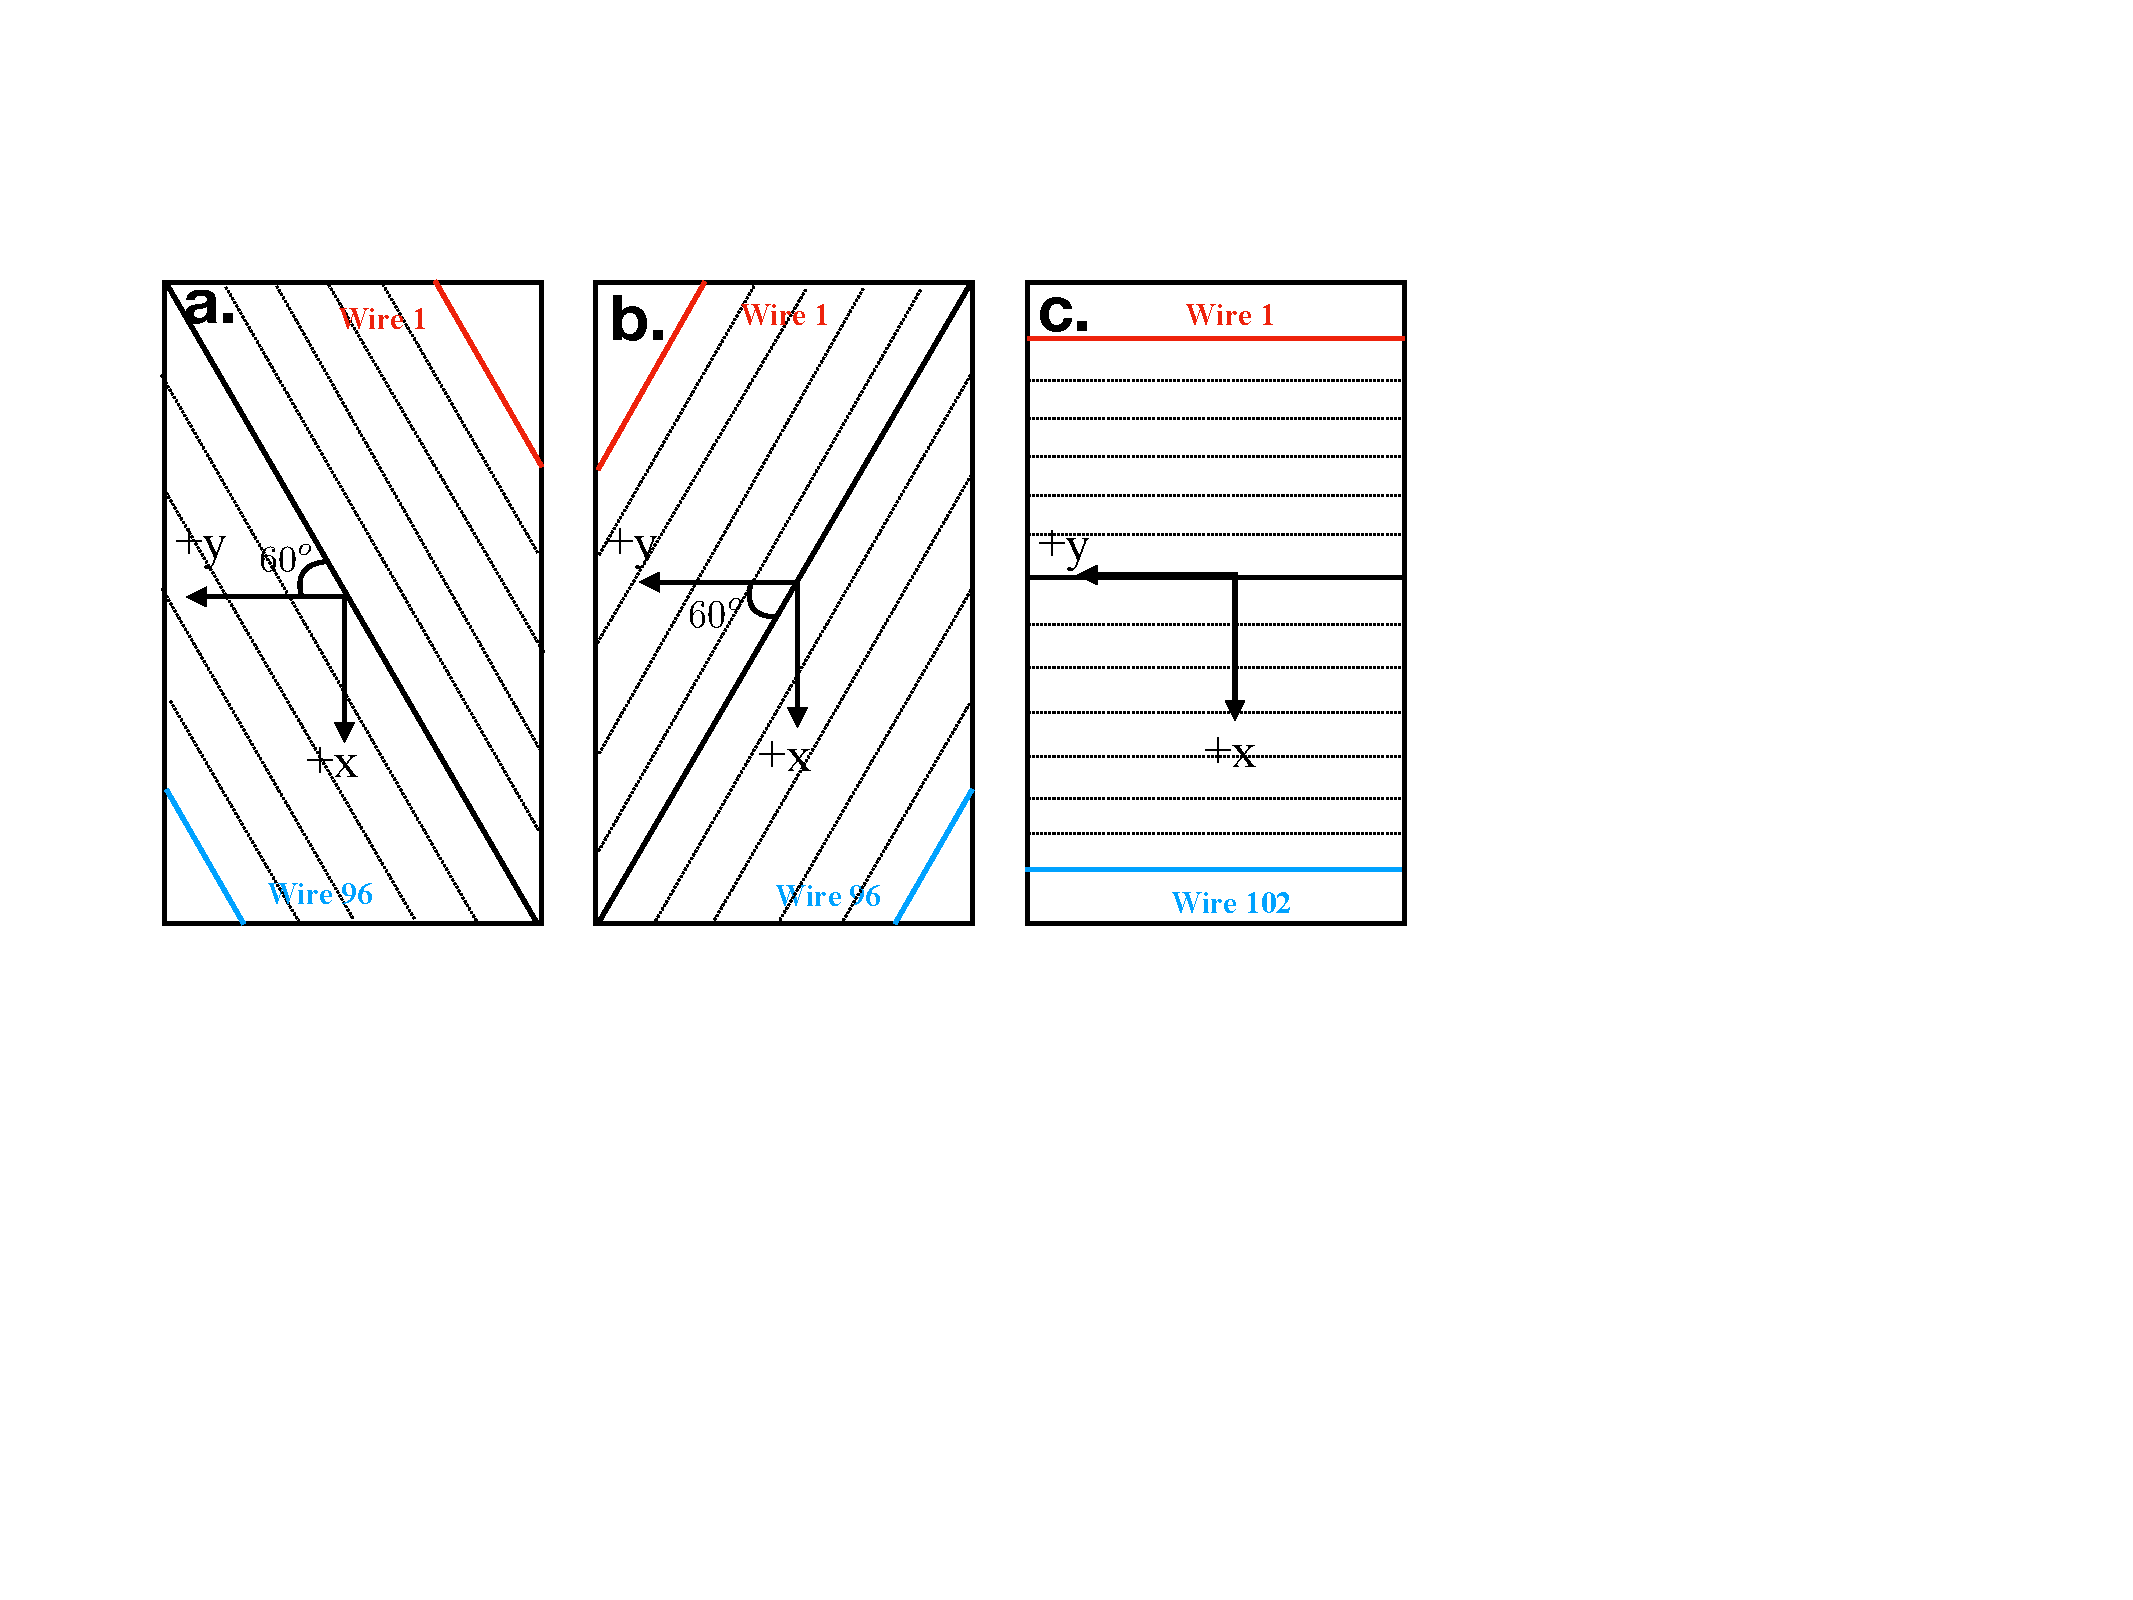
\includegraphics[width=3.0in, height=1.5in]{dc2_tests/HMS_DC_Wires.pdf}
  \caption{HMS Drift Chamber wire orientation for planes a) U, U', b) V, V' and c) X, X' where
  the direction of the beam (+z) is into the plane of the paper.}
  \label{fig:dc_wires}
\end{figure}\\
\indent The cathode planes and field wires are held at a negative high voltage and the sense wires are grounded which establishes a potential gradient causing an electric field
between high voltage and grounded wires. Each chamber is filled with a gas mixture\footnote{Argon is mixed with CO$_{2}$ or Ethane, where Argon is the ionizing agent the
particles interact with, and Ethane/CO$_{2}$ are the quenching elements to control avalanche produced by secondary ionization} of Argon with either CO$_{2}$ or Ethane.
As the particles traverse the chamber, the free electrons from ionized Argon drift towards the sense wires producing a detectable signal which is read out via discriminator
cards and into electronic modules.

\subsection{HMS Drift Chamber Cosmic Tests}
\noindent To determine the operatility of the HMS Drift Chambers, several cosmic tests were performed on the chambers in the Experimental Storage Building (ESB) before being transported
to Hall C. The chambers did not held the High Voltage beyond 1850 V without drawing a significant amount of current ($\geq$ 10 $\mu$A ) using a gas mixture of 75:25 Ar/CO$_{2}$ by
volume. When Drift Chamber II (DCII) was transported to Hall C, the gas mixture was changed to 50:50 Ar/Ethane and a High Voltage scan was done (See Figure \ref{fig:current_draw})  
\begin{figure}[h!]
  \centering
  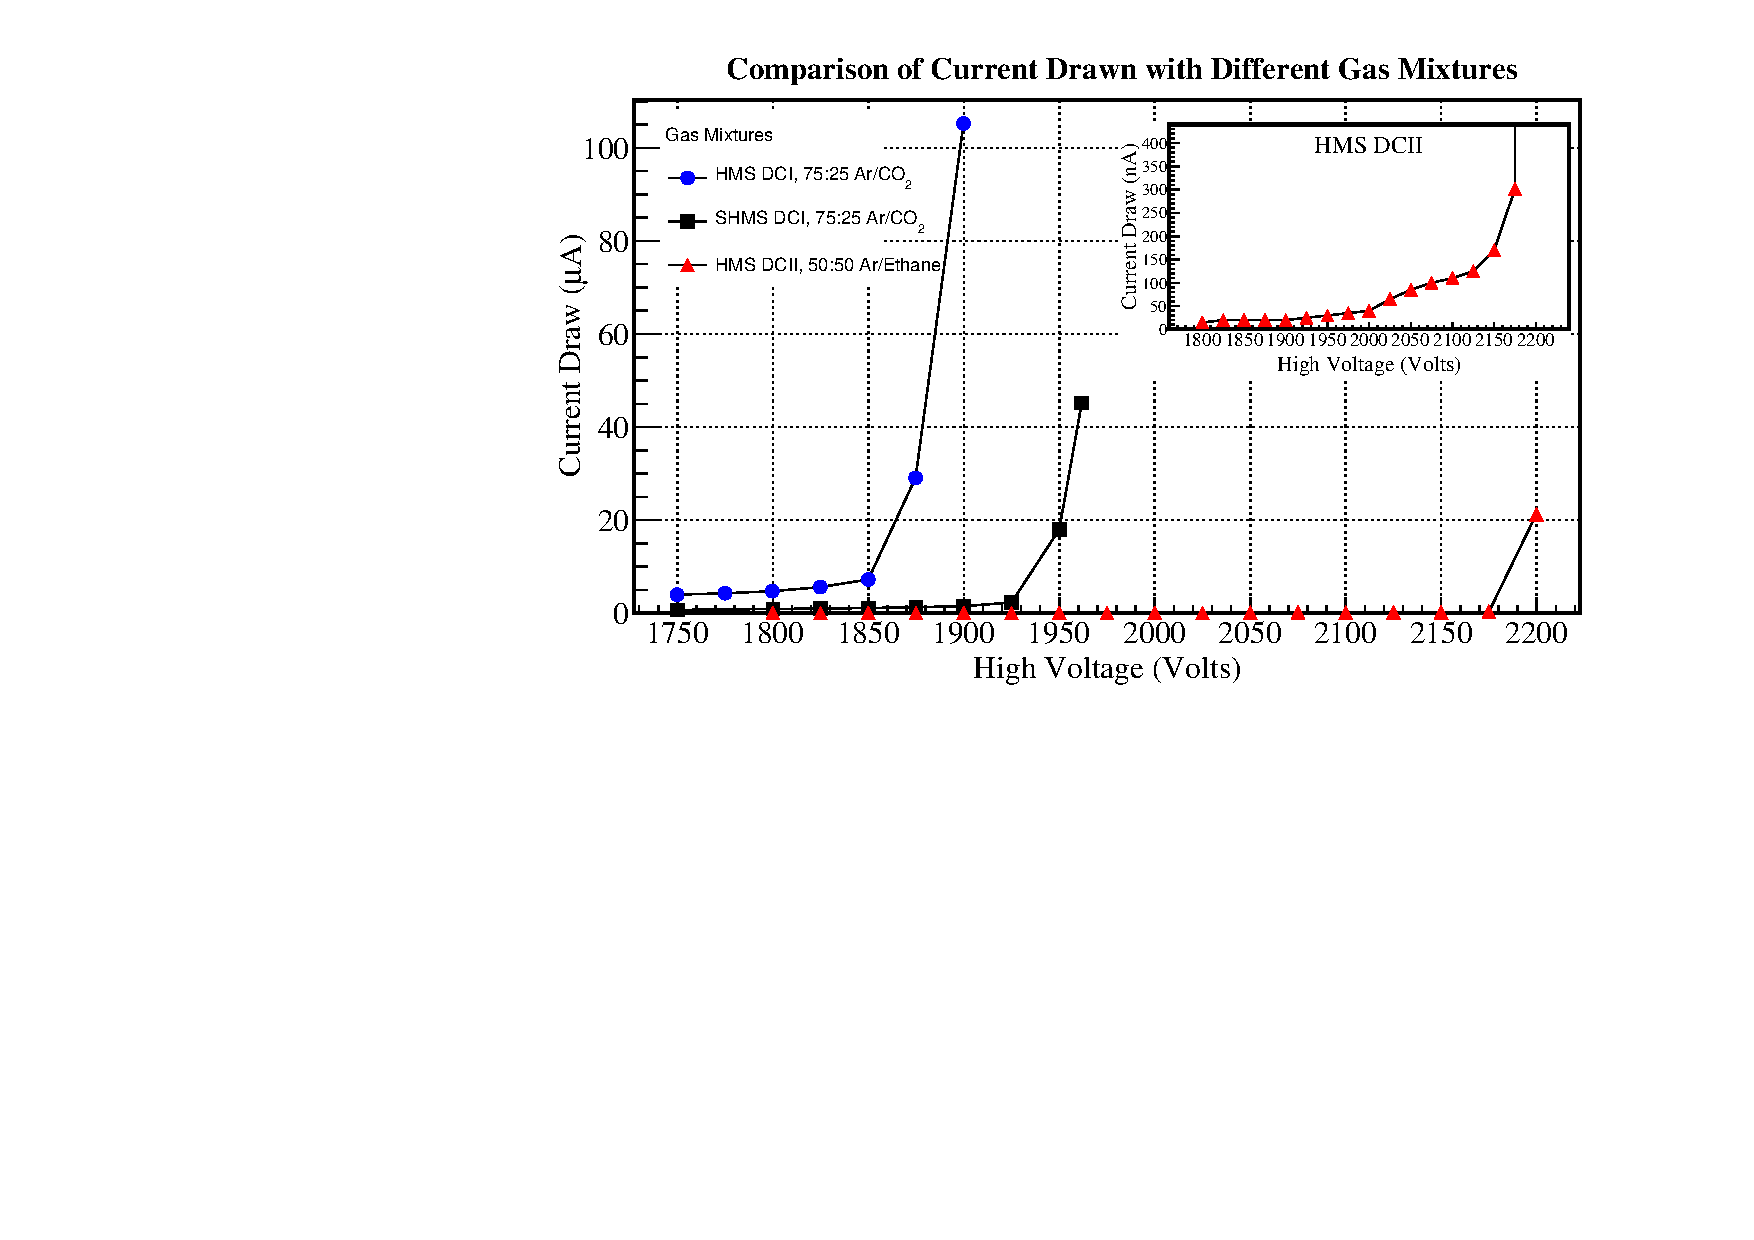
\includegraphics[width=3.5in, height=2.4in]{dc2_tests/gas_mix_current_drawn.pdf}
  \caption{Comparison of the current drawn in the HMS and SHMS chambers for different gas mixtures. The subplot shows a zoomed version of the Argon/Ethane gas mixture used in HMS DC II plot on a nanoampere scale.}
  \label{fig:current_draw}
\end{figure} \\
Figure \ref{fig:current_draw} shows a decrease in the current drawn by the HMS chambers by three orders of magnitude smaller, from a few $\mu$A to a few nA of current drawn. This
indicates that Ethane is a better quenching gas, as it kept the secondary electron ionization small for a broader range of High Voltages, up to $\sim$2100 Volts. There is still the
unresolved issue of why the HMS and SHMS chambers behave differently with the same gas mixture, since they both have the same design. The broad High Voltage range achieved by DC II without
significant current drawn allows for a better determination of the \textit{Plateau Region} of the chambers, which is a region in which the chamber efficiencies have little sensitivity
to relatively large High Voltage variations. \\
\indent To determine the plateau region of HMS DC II,  a cosmic test stand was set up in the HMS detector hut (See Figure \ref{fig:cosmic_stand}). The setup consists of two scintillator paddles on the top
and two on bottom of the chamber. The top two are completely overlapped while the bottom two are only partially overlapped. Each scintillator paddle is wrapped around a light tight material known as Tedlar,
and is coupled to a Photomultiplier Tube (PMT) via a light guide. To ensure that only cosmic rays pass through the chamber, a coincidence between the top and bottom PMTs is made. It is required that the top
two PMTs detect a signal to reduce the probability of instrinsic noise being interpreted as a cosmic signal. The bottom scintillators are partially overlapped to achieve full coverage of the chamber active
area, and a less restrictive requirement was made by requiring that either of the bottom PMTs detect a signal. A final requirement was made so that the top and bottom PMTs would detect a signal within a
certain time window. This requirement ensures a correlation between the top and bottom PMT signals, making it highly probable that the signal was produced by a cosmic ray. The correlated signal between the top and
bottom PMTs is defined as the \textit{trigger}. The efficiency of the \textit{i$^{th}$} plane, $\epsilon_{i}$, can then be defined as follows, \\
\begin{align*}
\epsilon_{i} = \frac{\# \text{ triggers that hit the \textit{i$^{th}$} plane } }{\# \text{ triggers that \textit{should} have hit the \textit{i$^{th}$} plane} } 
\end{align*} \\
given that the other five planes received at least one hit from the cosmic. \\
\indent To make a reliable efficiency measurement, it has to be ensured from the geometry of the cosmic set-up, that any cosmic passing though the top and bottom scintillators also traverses every plane in the chamber
to make the efficiency measurements unbiased to the scintllators orientation. 
\begin{figure}[h!]
  \centering
  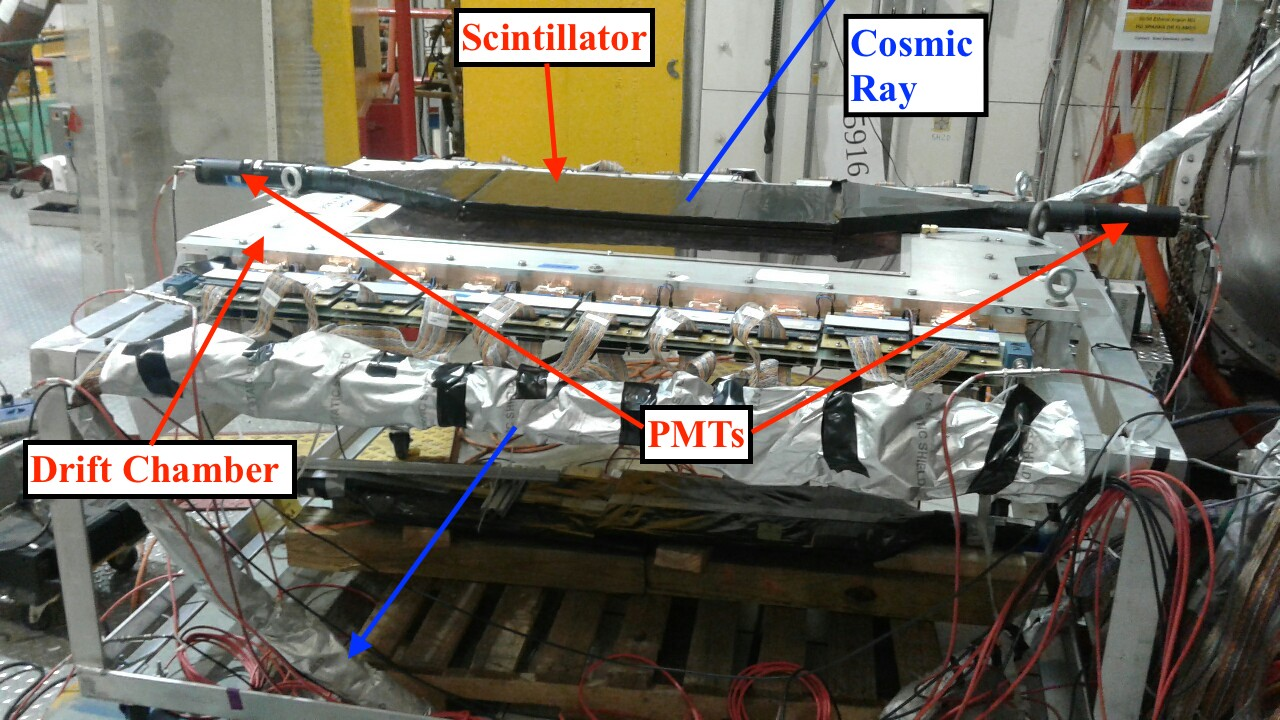
\includegraphics[width=3.4in, height=2.4in]{dc2_tests/dc2_teststand_03.jpg}
  \caption{Cosmic test stand setup in Hall C detector hut.}
  \label{fig:cosmic_stand}
\end{figure} \\
When cosmic data was taken, to ensure that all (or at least most) of the sense wires in each plane were present (and had not been damaged by transporting the chamber), the wiremap distribution was
a looked at first. The distributions show full occupancy for all wire planes in DC II (See Figure \ref{fig:hdc2_wiremap}).  
\begin{figure}[h!]
  \centering
  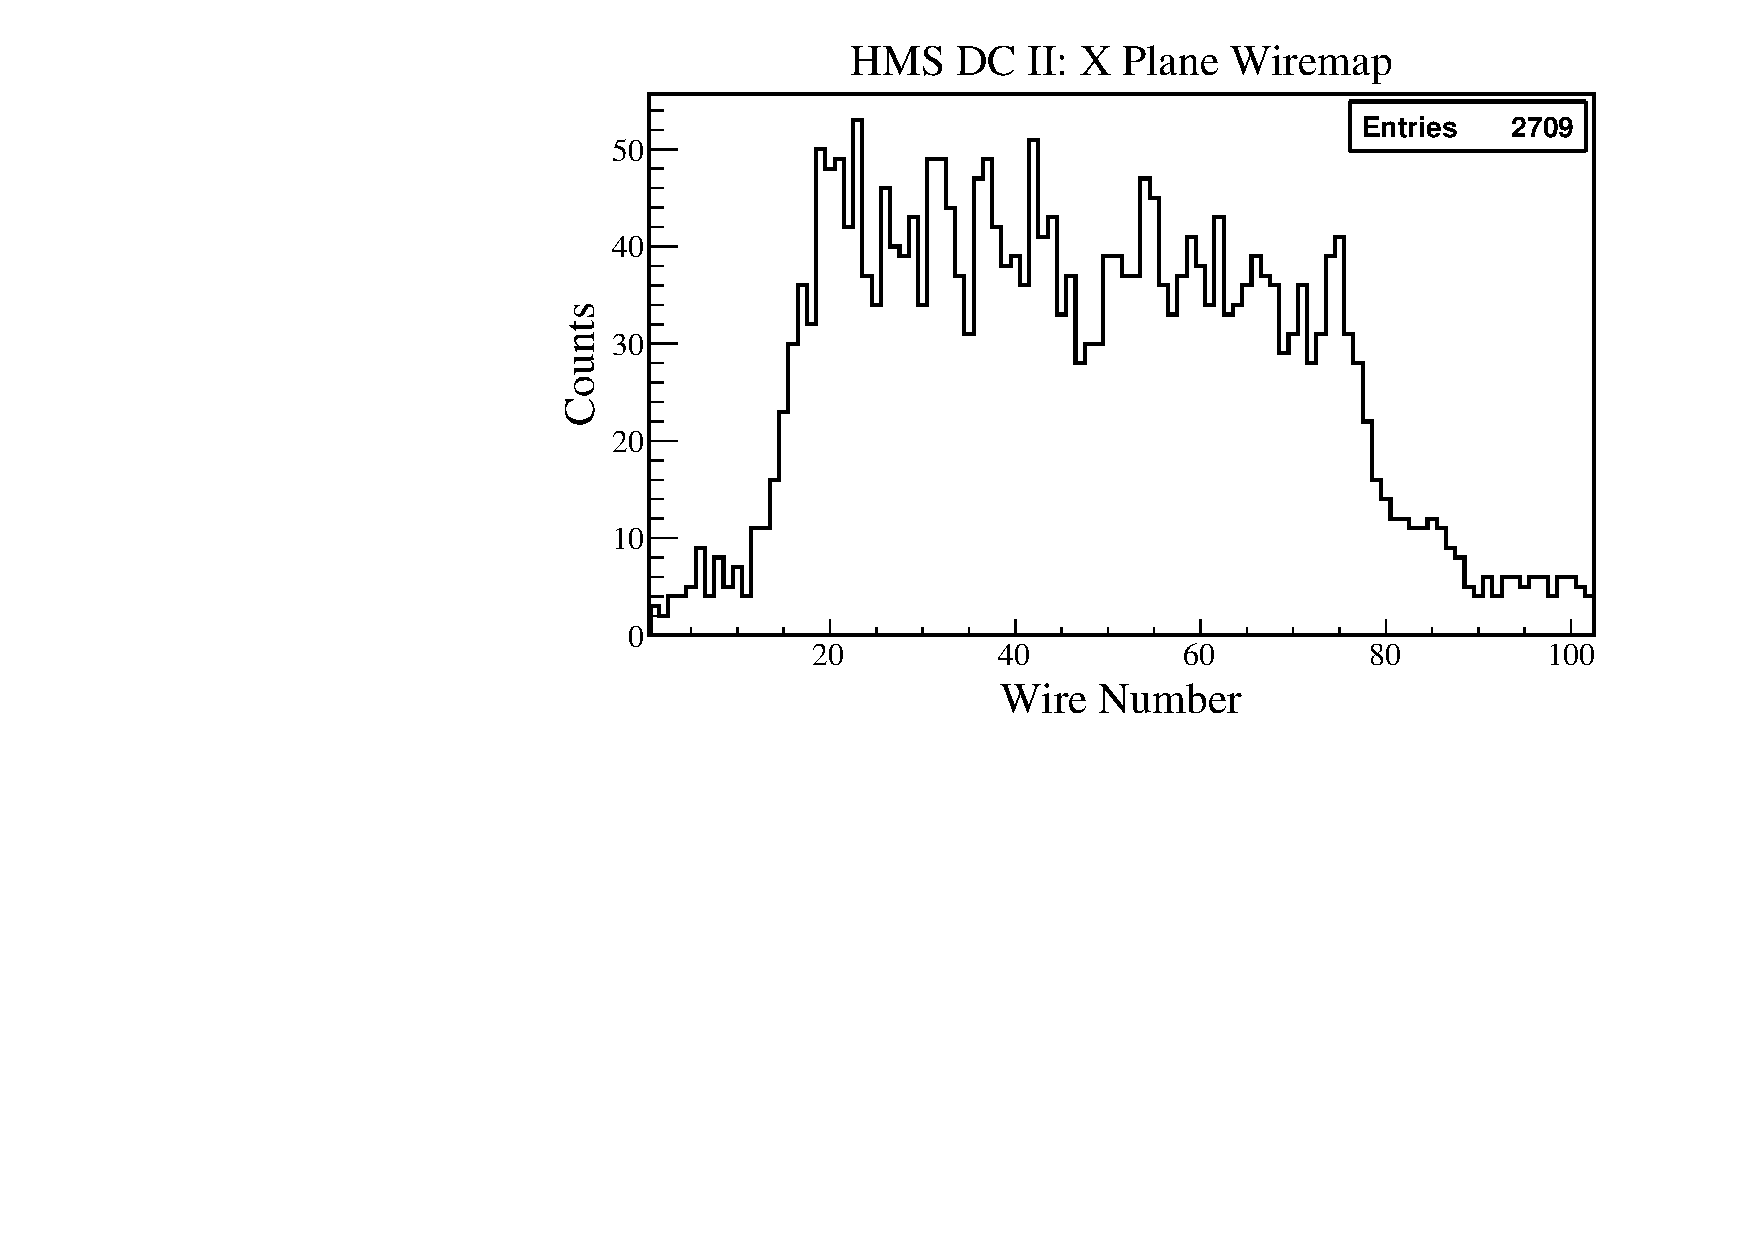
\includegraphics[width=3.7in, height=2.2in]{dc2_tests/hdc2_xmap.pdf}
  \caption{Wiremap distribution of the X Plane in DC II shows occupancy in all wires.}
  \label{fig:hdc2_wiremap}
\end{figure} \\
Once all planes of the chamber were verified to have full occupancy, a High Voltage and threshold\footnote{The threshold set on the chamber is used to filter cosmic signals from noise by requiring 
the signal amplitude to cross a threshold before discriminating them to produce logic signals, which are read out by the electronic modules.} scan was done to determine the plateau region. A high voltage scan was done first
by setting the threshold fixed at 4.5 V to determine the optimal HV setting. A threshold scan was then performed at 1940 V to determine the optimal threshold. The results are shown in Figures \ref{fig:hdc2_hvscan}
and \ref{fig:hdc2_thrsscan}. The high voltage scan in Figure \ref{fig:hdc2_hvscan} shows the plateau region starting at 1900 V. The chamber operational high voltage was chosen to be 1940 V since the efficiencies seem
to be stable and better than 99$\%$ over a $\sim\pm$40 Volt range about this central setting.
\begin{figure}[h!]
  \centering
  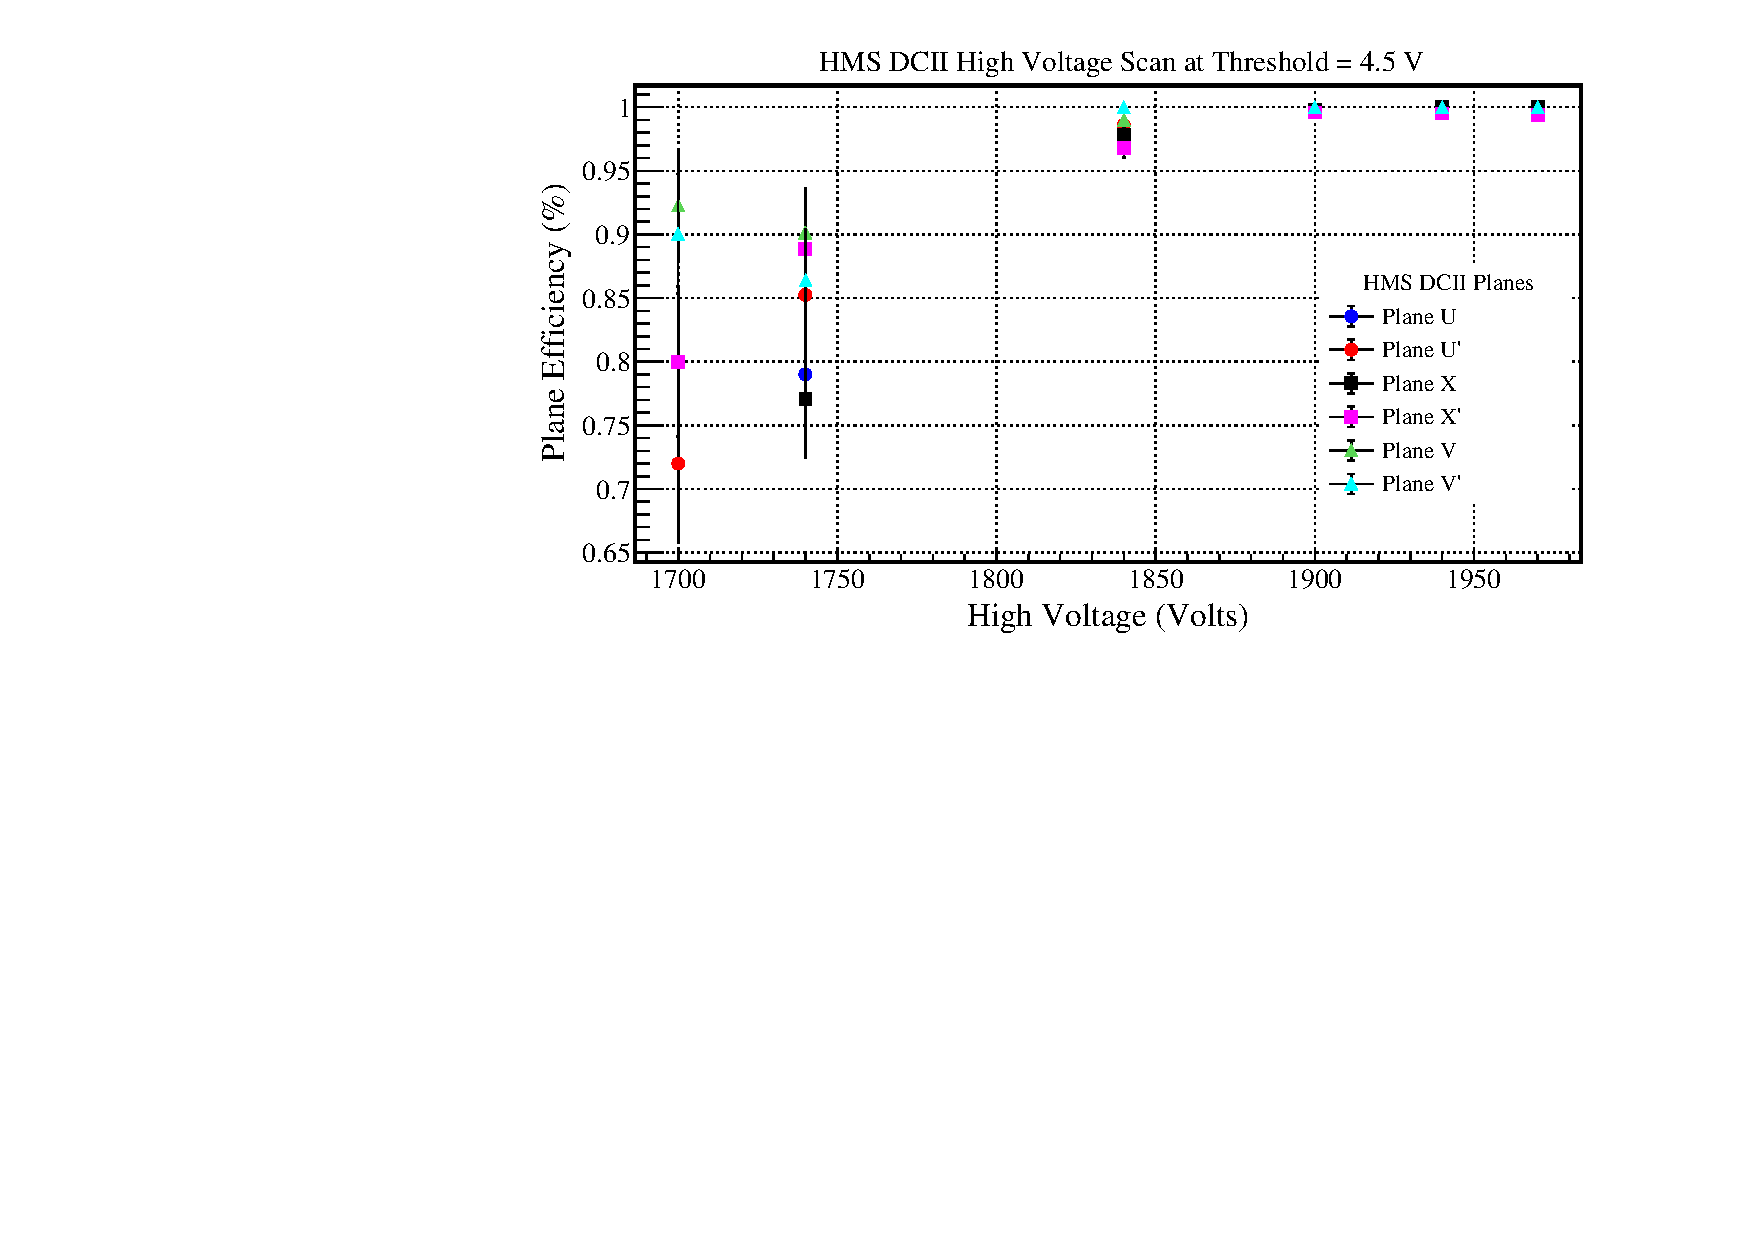
\includegraphics[width=3.8in, height=2.2in]{dc2_tests/dc2_hvscan_thrs45.pdf}
  \caption{High Voltage scan of DC II over a broad range at a Threshold of 4.5 Volts.}
  \label{fig:hdc2_hvscan}
\end{figure} 
\begin{figure}[h!]
  \centering
  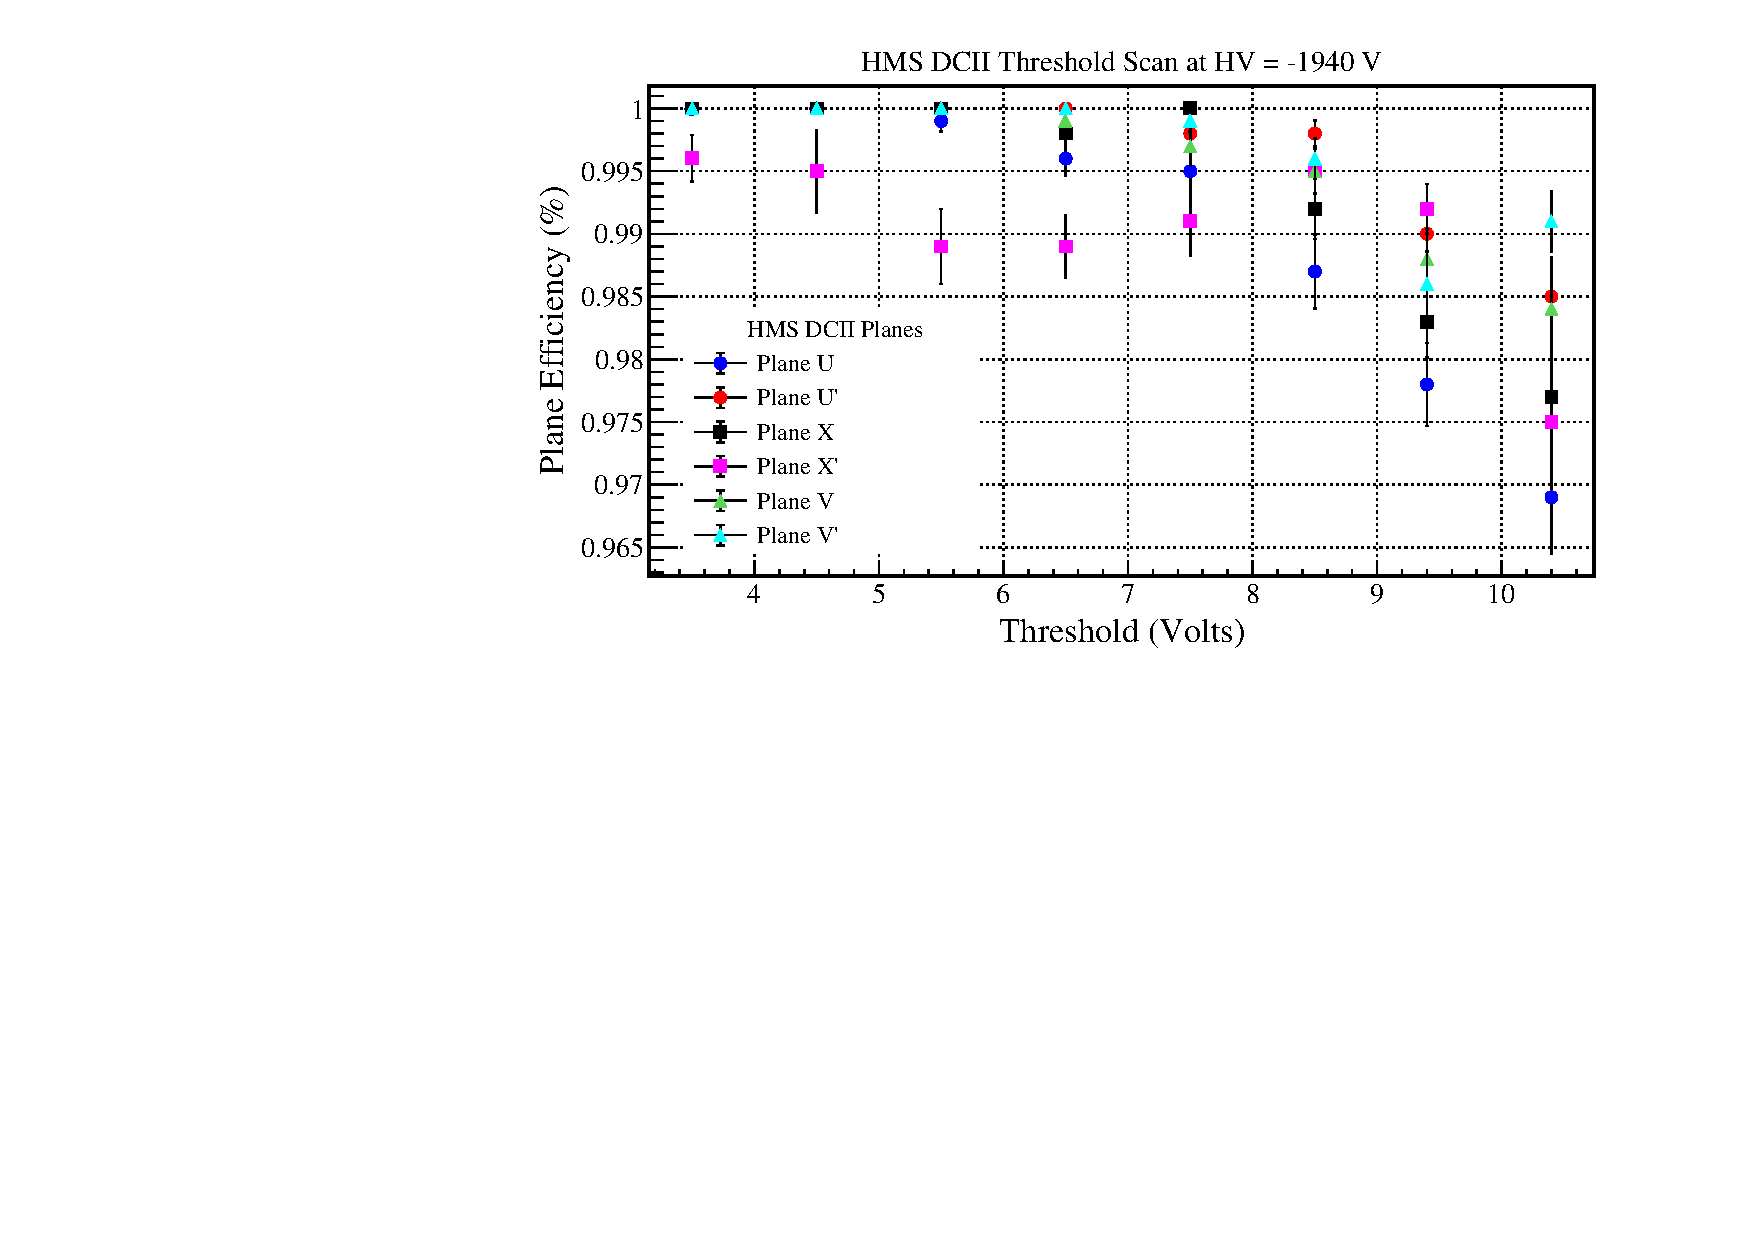
\includegraphics[width=3.8in, height=2.2in]{dc2_tests/dc2_thrsscan_HV_1940V.pdf}
  \caption{Threshold scan over a broad range at a HV setting of 1940 V.}
  \label{fig:hdc2_thrsscan}
\end{figure} \\
\indent From the threshold scan results in Figure \ref{fig:hdc2_thrsscan}, there is a 3$\%$ decrease in the plane efficiencies over a
6 Volt range. The operational threshold voltage was determined to be 4.5 Volts, where the efficiencies are better than 99$\%$, over a $\sim$ 1 Volt range.
The high voltage and threshold settings determined from the scans were chosen based on the high efficiency region and its small sensitivity over a voltage range.  


\section{Electronic and Computer Deadtime Studies}
\subsection{Dead Time Measurements Procedure}
\noindent The procedure to determine the computer and electronic dead times is currently in the development stage in Hall C. The general idea is to use a pulse generator to produce
a fixed frequency pulse and feed it as early as possible into the electronic modules being used in the experimental setup. This pulse will interfere wth the actual signals
produced by physics, but its rate can be set orders of magnitude smaller such that its interference will be minimal and will have insignificant contribution to the deadtime.
By counting the number of pulses generated before sending them to the electronics chain, compared to the number of pulses that actually make it to the end of the chain and
are accepted by the TI (Trigger Interface) module\cite{TI}, one may determine the dead time as follows:
\begin{equation} \label{deadtime}
  \text{total D.T.} = 1 - \underbrace{\frac{\# \text{ of accepted pulses}}{\# \text{ of generated pulses}}}_{\text{\normalsize total L.T.}} 
\end{equation}
This is the total deadtime from the electronics and computer (TI module) that arises due to the finite processing time of the modules. From Eq. \ref{deadtime},  the total live time has contributions from the computer and electronics, which can
be calculated separately. \\
\indent The computer live time is calculated by the TI module since it has an
internal scaler which counts the number of input and accepted triggers, and takes the ratio. This calculation can also be done externally as a cross-check by counting the number of signals that make it to the
TI via an external scaler module, and comparing it to the number of accepted triggers which is outputted by the TI and determined during the data analysis stage. \\
\indent The electronics livetime cannot be determined directly,  but it can be determined by keeping the computer live time fixed near 100$\%$ and
increasing the pulse generator rate to probe the capability of the electronics modules to handle high rates. This way, if there is a decrease in the total live time which can be measured directly, then it must have been caused by the
electronics, since the computer live time is kept fixed. \\
\indent One might argue that such high rates can reduce the computer live time itself which is true, however, such high rates can be pre-scaled by the TI by orders
of magnitude, such that the computer live time is kept fixed. For example, the TI can be pre-scaled by 10$^{2}$ such that for a rate of 100,000 counts/sec. (100 KHz), the TI accepts 1 kHz.  Using this technique, one can investigate the
effects of high rates on the electronic modules without having a significant contribution from the computer live time. \\
\subsection{Basic Concepts on Computer Live Time}
\noindent To better understand how the computer live time is determined, I will introduce some basic concepts about how the TI module does this calculation. The main functionality of the TI is to process and distribute triggers and initiate data readout in fast electronics modules. Due to the finite processing time of these modules, the TI has a \textit{deadtime} in which it is unable to process any more triggers until after all other fast electronics modules have finished processing the current trigger. During this time, the TI generates a BUSY signal typically on the order of a few microseconds ($\mu$s) during which
all other input triggers are rejected. \\
\indent To understand computer live time experimentally, one can use a pulse generator to feed a controlled pulse into the TI and explore the effect of
various pulse rates on the deadtime. Based on the periodicity of the input pulse and the output BUSY signal width of the TI, three limiting cases arise:
\begin{figure}[h!]
  \centering
  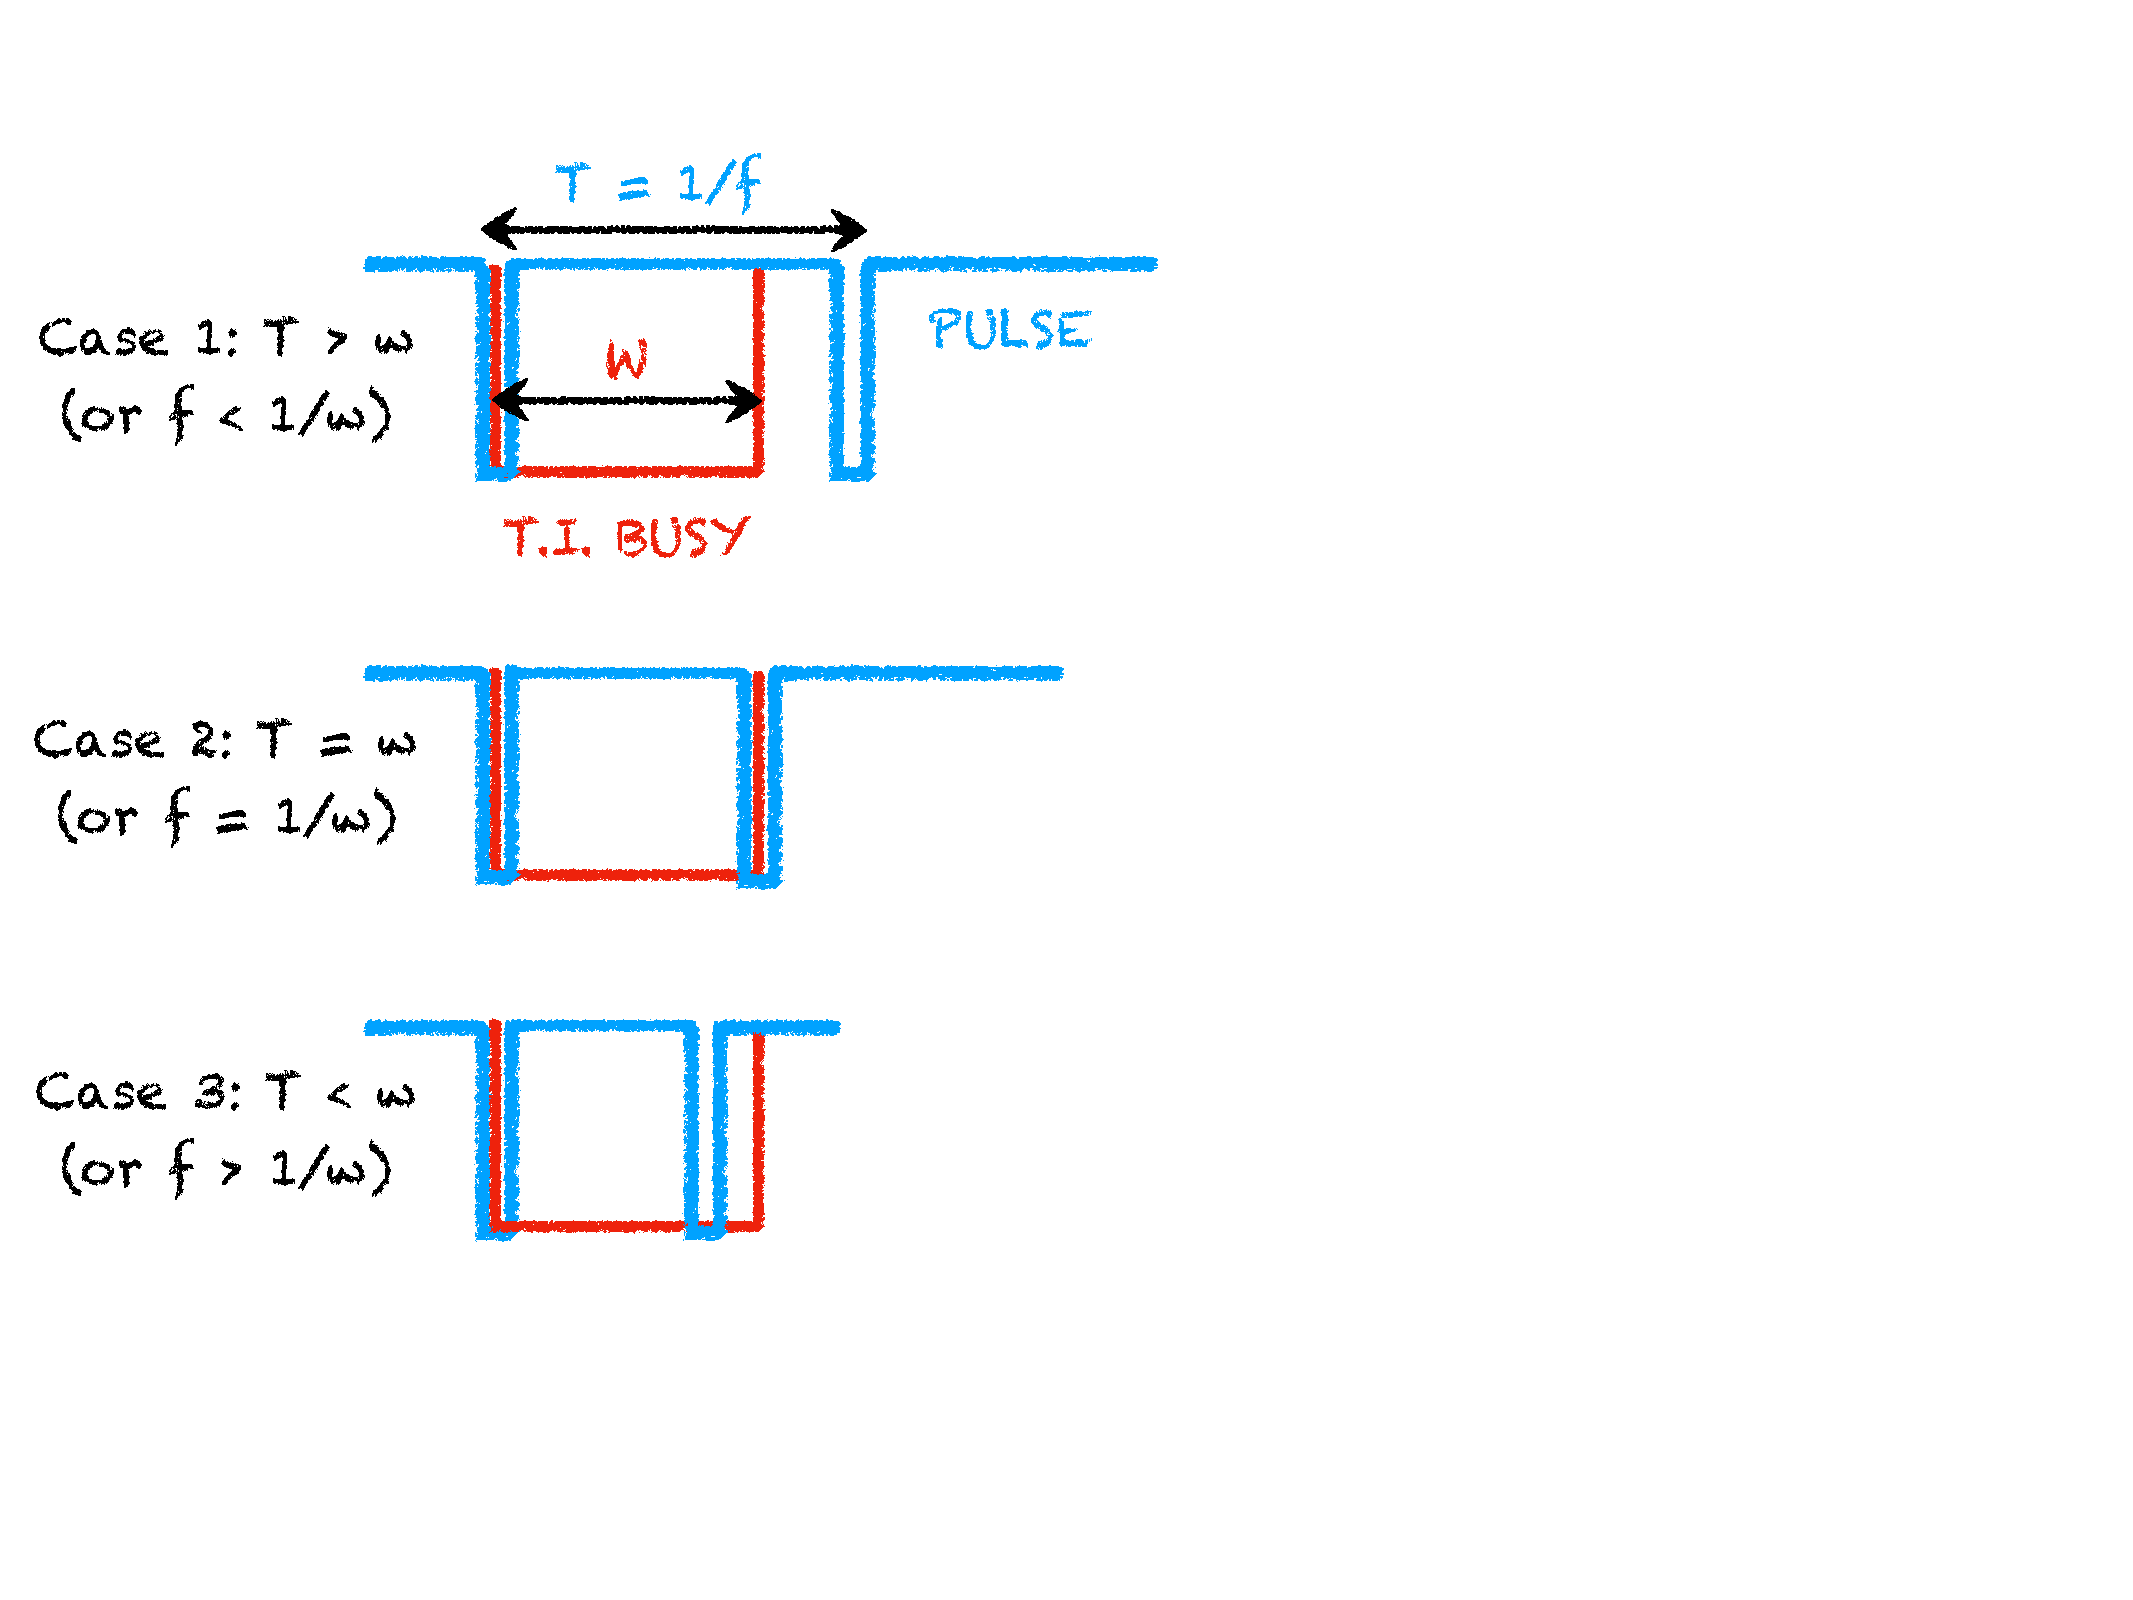
\includegraphics[width=3.4in, height=2.8in]{edtm/edtm_cases.pdf}
  \caption{Three limiting cases on TI computer live time based on the input signal.}
  \label{fig:edtm_cases}
\end{figure} \\

\begin{itemize}
\item Case 1: The pulse periodicity falls outside the TI BUSY window so the ratio of accepted signals to input signals is unity and the live time is 100$\%$\\
\item Case 2: The pulse periodicity is equal to the width of the BUSY window, so every two input pulses, the first one wll open a BUSY window and the second will be blocked by the BUSY so the TI accepts only 1/2 the input signals and the live time is 50$\%$. \\
\item Case 3: The pulse periodicity is smaller than the BUSY window so the live time is 50$\%$ or less. 
\end{itemize}
For the second and third case, a general expression for the computer live time can be obtained by expressing the pulse periodicity $T$ as a fraction
of the BUSY width, $w$. For a pulse period
\begin{equation}\label{eq:period}
T = \frac{1}{n}w, \text{ where n = 1, 2, 3, . . .} 
\end{equation}
the computer live time can be shown to be 
\begin{equation}\label{eq:L.T.}
 \text{computer L.T. } = \frac{1}{n+1}
\end{equation}
For example, if the period is one-half of the BUSY width, then the first pulse that comes initiates the BUSY, the second pulse will arrive half way, and
the third pulse will be at the end of the BUSY, so only 1/3 (33$\%$ live time) of the pulses will be accepted by the TI as the other two will be rejected since they did
not arrived outside the window. \\
\indent In the previous discussions, I have used the example of a pulse generator that produces periodic pulses in time. In reality, during a physics experiment, the physics events
that are detected follow poisson statistics, which is a random process. This means that pulses arrive random in time, and so it becomes impossible to predict exactly what the computer
live time will be (See Figure \ref{fig:poisson_pulse}).
\begin{figure}[h!]
  \centering
  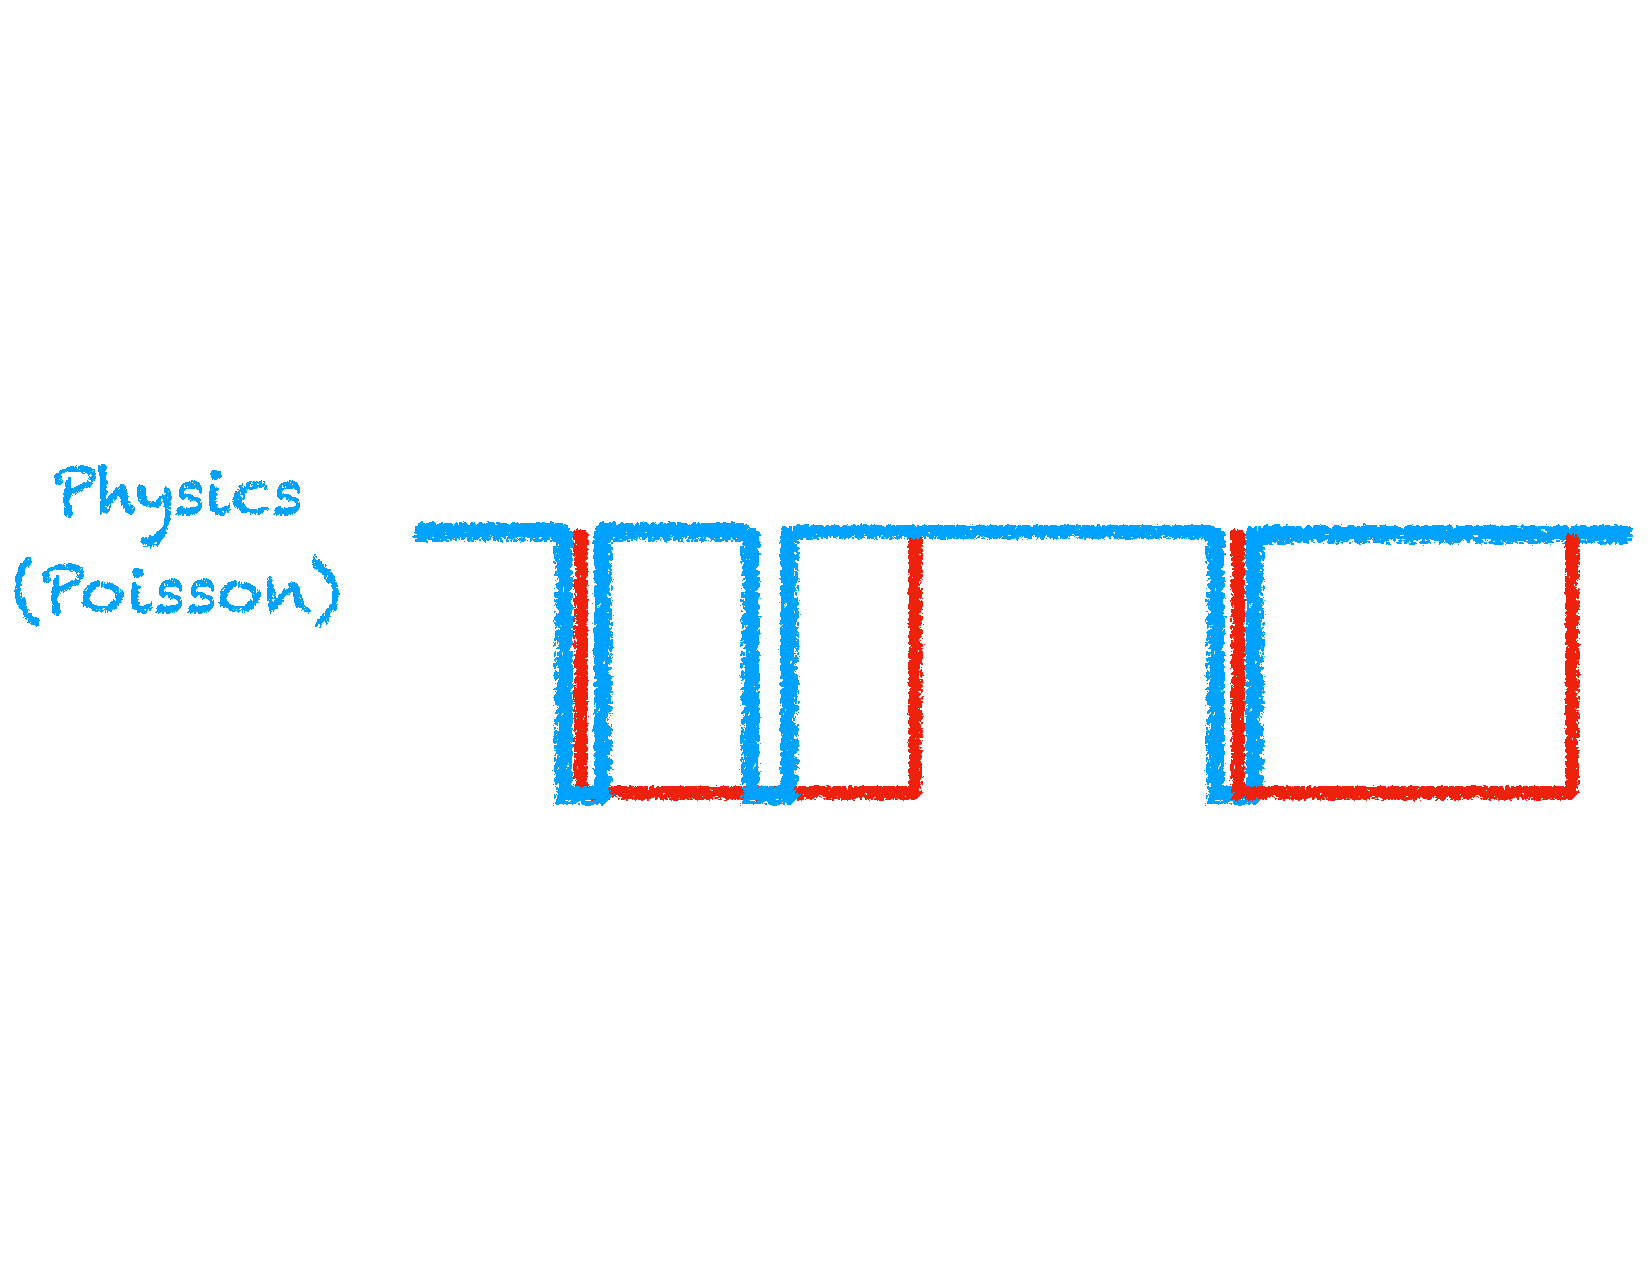
\includegraphics[width=3.1in, height=0.9in]{edtm/poisson_pulse.pdf}
  \caption{Random pulses in time due to physics events follow poisson statistics.}
  \label{fig:poisson_pulse}
\end{figure}\\
In Figure \ref{fig:poisson_pulse}, the first pulse initiates a BUSY signal, the following pulses then arrive at random times which may or may not be within the BUSY width so achieving a live
time of 100$\%$ becomes highly improbable during an experimental run.
\subsection{Computer Live Time Measurements}
\noindent Initial measurements of the computer live time were performed and the results of these measurements uncovered several issues associated with the
TI module and the DAQ which required the help from experts. The first set of measurements were done using a pulse generator at various rates up to 10 kHz. The pulses were fed to the electronics modules in both the HMS and SHMS and the BUSY signal widths were measured. The results are shown in Table \ref{table:cp_LT}. \\ 
\begin{table}[ht]
\caption{Measured Computer Live Times with Pulse Generator}
\centering
{\def\arraystretch{1.6}\tabcolsep=5pt
\begin{tabular}{c c c c}
\hline\hline
Pulse Rate & HMS & SHMS & BUSY width \\ [0.5ex] % inserts table %heading
\hline
100 Hz & 98.85$\%$ & 99.84 $\%$ &HMS: 2.2 ms \\
500 Hz & 50.07$\%$ & 98.30 $\%$  &SHMS: 2.2 $\mu$s \\
1 kHz  & 33.44$\%$ & 99.21 $\%$  \\
5 kHz  & 8.33$\%$ & 45.2 $\%$ \\
10 kHz & 4.30$\%$ & 30.49 $\%$ \\ [1ex]
\hline
\end{tabular}
}
\label{table:cp_LT}
\end{table} 
\indent From Eqs. \ref{eq:period} and \ref{eq:L.T.}, and the BUSY widths in Table \ref{table:cp_LT}, the expected computerlive times for certain frequencies can be calculated and the results are shown in
Tables \ref{table:expected_hmscp_LT} and \ref{table:expected_shmscp_LT}. \\
\begin{table}[ht]
\caption{Expected HMS Computer Live Times with Pulse Generator}
\centering
{\def\arraystretch{1.6}\tabcolsep=5pt
\begin{tabular}{c c c}
\hline\hline
($T=\frac{1}{n}w$) & Pulse Rate ($f = \frac{1}{T}$) & HMS ($\frac{1}{1+n}$) \\ [0.5ex] % inserts table %heading
\hline
$>w$             & $<$ 500 Hz & 100 $\%$ \\
$w$              & 500 Hz & 50  $\%$ \\
$\frac{1}{2}w$   & 1 kHz & 33.3 $\%$  \\
$\frac{1}{4}w$   & 2 kHz & 20.0 $\%$  \\
$\frac{1}{10}w$  & 5 kHz & 9.09 $\%$ \\
$\frac{1}{20}w$  & 10 kHz & 4.76 $\%$ \\ [1ex]
\hline
\end{tabular}
}
\label{table:expected_hmscp_LT}
\end{table} 
\begin{table}[ht]
\caption{Expected SHMS Computer Live Times with Pulse Generator}
\centering
{\def\arraystretch{1.6}\tabcolsep=5pt
\begin{tabular}{c c c}
\hline\hline
($T=\frac{1}{n}w$) & Pulse Rate ($f = \frac{1}{T}$) &  SHMS ($\frac{1}{1+n}$) \\ [0.5ex] % inserts table %heading
\hline
$>w$             & $<$ 454 kHz & 100 $\%$ \\
$w$              & 454 kHz & 50  $\%$ \\
$\frac{1}{2}w$   & 909 kHz & 33.3 $\%$  \\
$\frac{1}{4}w$   & 1.81 MHz & 20.0 $\%$  \\ [1ex]
\hline
\end{tabular}
}
\label{table:expected_shmscp_LT}
\end{table} 
\indent A comparison between the expected and measured computer live times in the HMS shows a discrepancy of $<$1$\%$ for rates $>500$Hz.
In the SHMS, however, since the BUSY signal is 10$^{3}$ orders of magnitude smaller than the HMS, a much high rate of 454 kHz is
expected before a dropping below 100$\%$ computer live times. Since the maximum rate measured in the SHMS was only 10 kHz, it was
expected that computer live times should have stayed at 100$\%$, but this was not the case. \\
\indent In addition to these measurements, to simulate physics events, a poisson pulse generator was also used to observe the
effects on the computer live times and view the signals on the Oscilloscope for instructional purposes (See Figure \ref{fig:scope_edtm}), but extensive measurements were
not done since the discrepancy between expected and measured livetimes using a pulse generator was a significant problem that needed to be
resolved. 
\begin{figure}[h!]
  \centering
  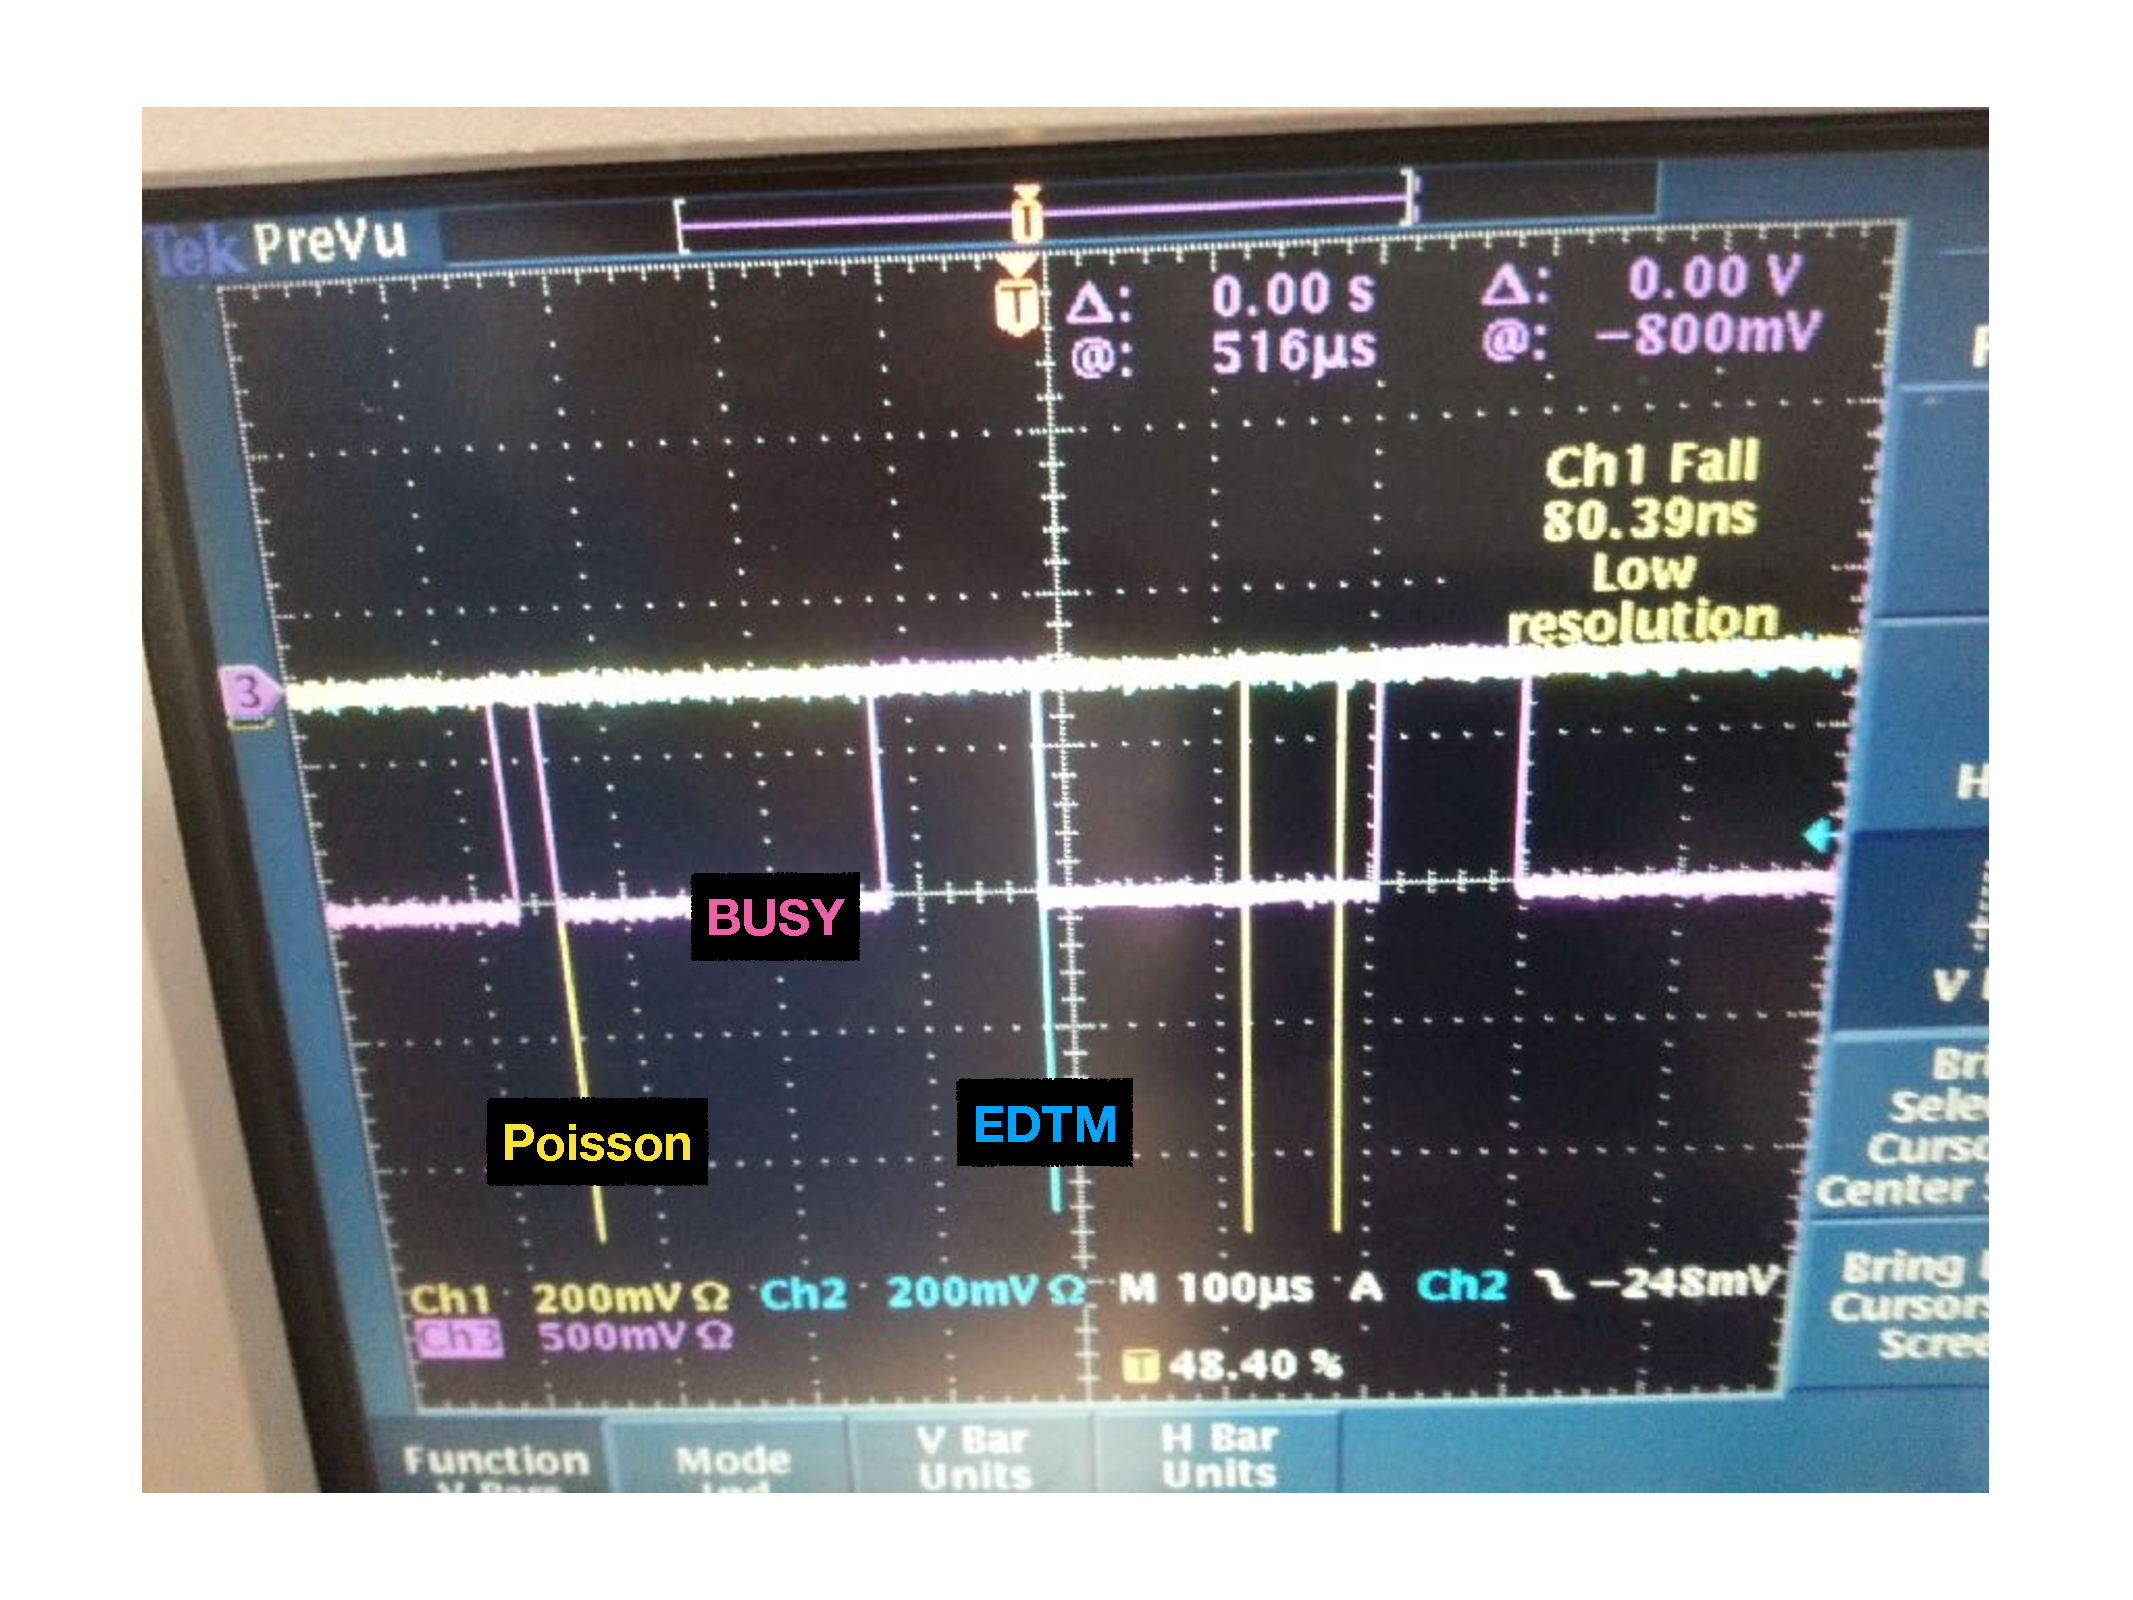
\includegraphics[width=3.4in, height=2.6in]{edtm/EDTM_Oscope.pdf}
  \caption{Random (Poisson) and periodic (EDTM - elecreonic dead time monitoring) pulses initiating a TI BUSY as viewed in an
    Oscilloscope. The pulses appear as a line because the horizontal scale is set to 100 $\mu$s / division, and the pulses have
  widths on the order of tens of nanoseconds, so they appear $10^{3}$ smaller.}
  \label{fig:scope_edtm}
\end{figure}\\
Figure \ref{fig:scope_edtm} is a visual representation of how the TI module responds to various input signals. The yellow signals were produced by
a random pulse generator to replicate physics events, and the blue pulse is periodic. The first pulse (yellow) initiates a BUSY (pink) signal from the
TI, but no other signals arrived during that time. A second pulse (blue) initiates a second BUSY signals, and during the 220 $\mu$s that the window
is open, two other random pulses arrived, but are rejected by the TI BUSY, since the other pulse was still being processed.

\subsection{Technical Issues with the DAQ and Trigger Interface Module}
\noindent The discrepancies found in the computer live times using periodic pulse generator shed light on unknown problems regarding the DAQ and TI
module that required the intervention of experts. One of the problems had to do with SYNCHRONIZATION issues between the TI and external scaler modules
which are used to count triggers. When taking experimental data, one must go over a series of steps in order to initiate and end the run. These steps
involve the communication between the TI and Scaler modules during a START/END of run processes (See Figure \ref{fig:TI_sync}). 
\begin{figure}[h!]
  \centering
  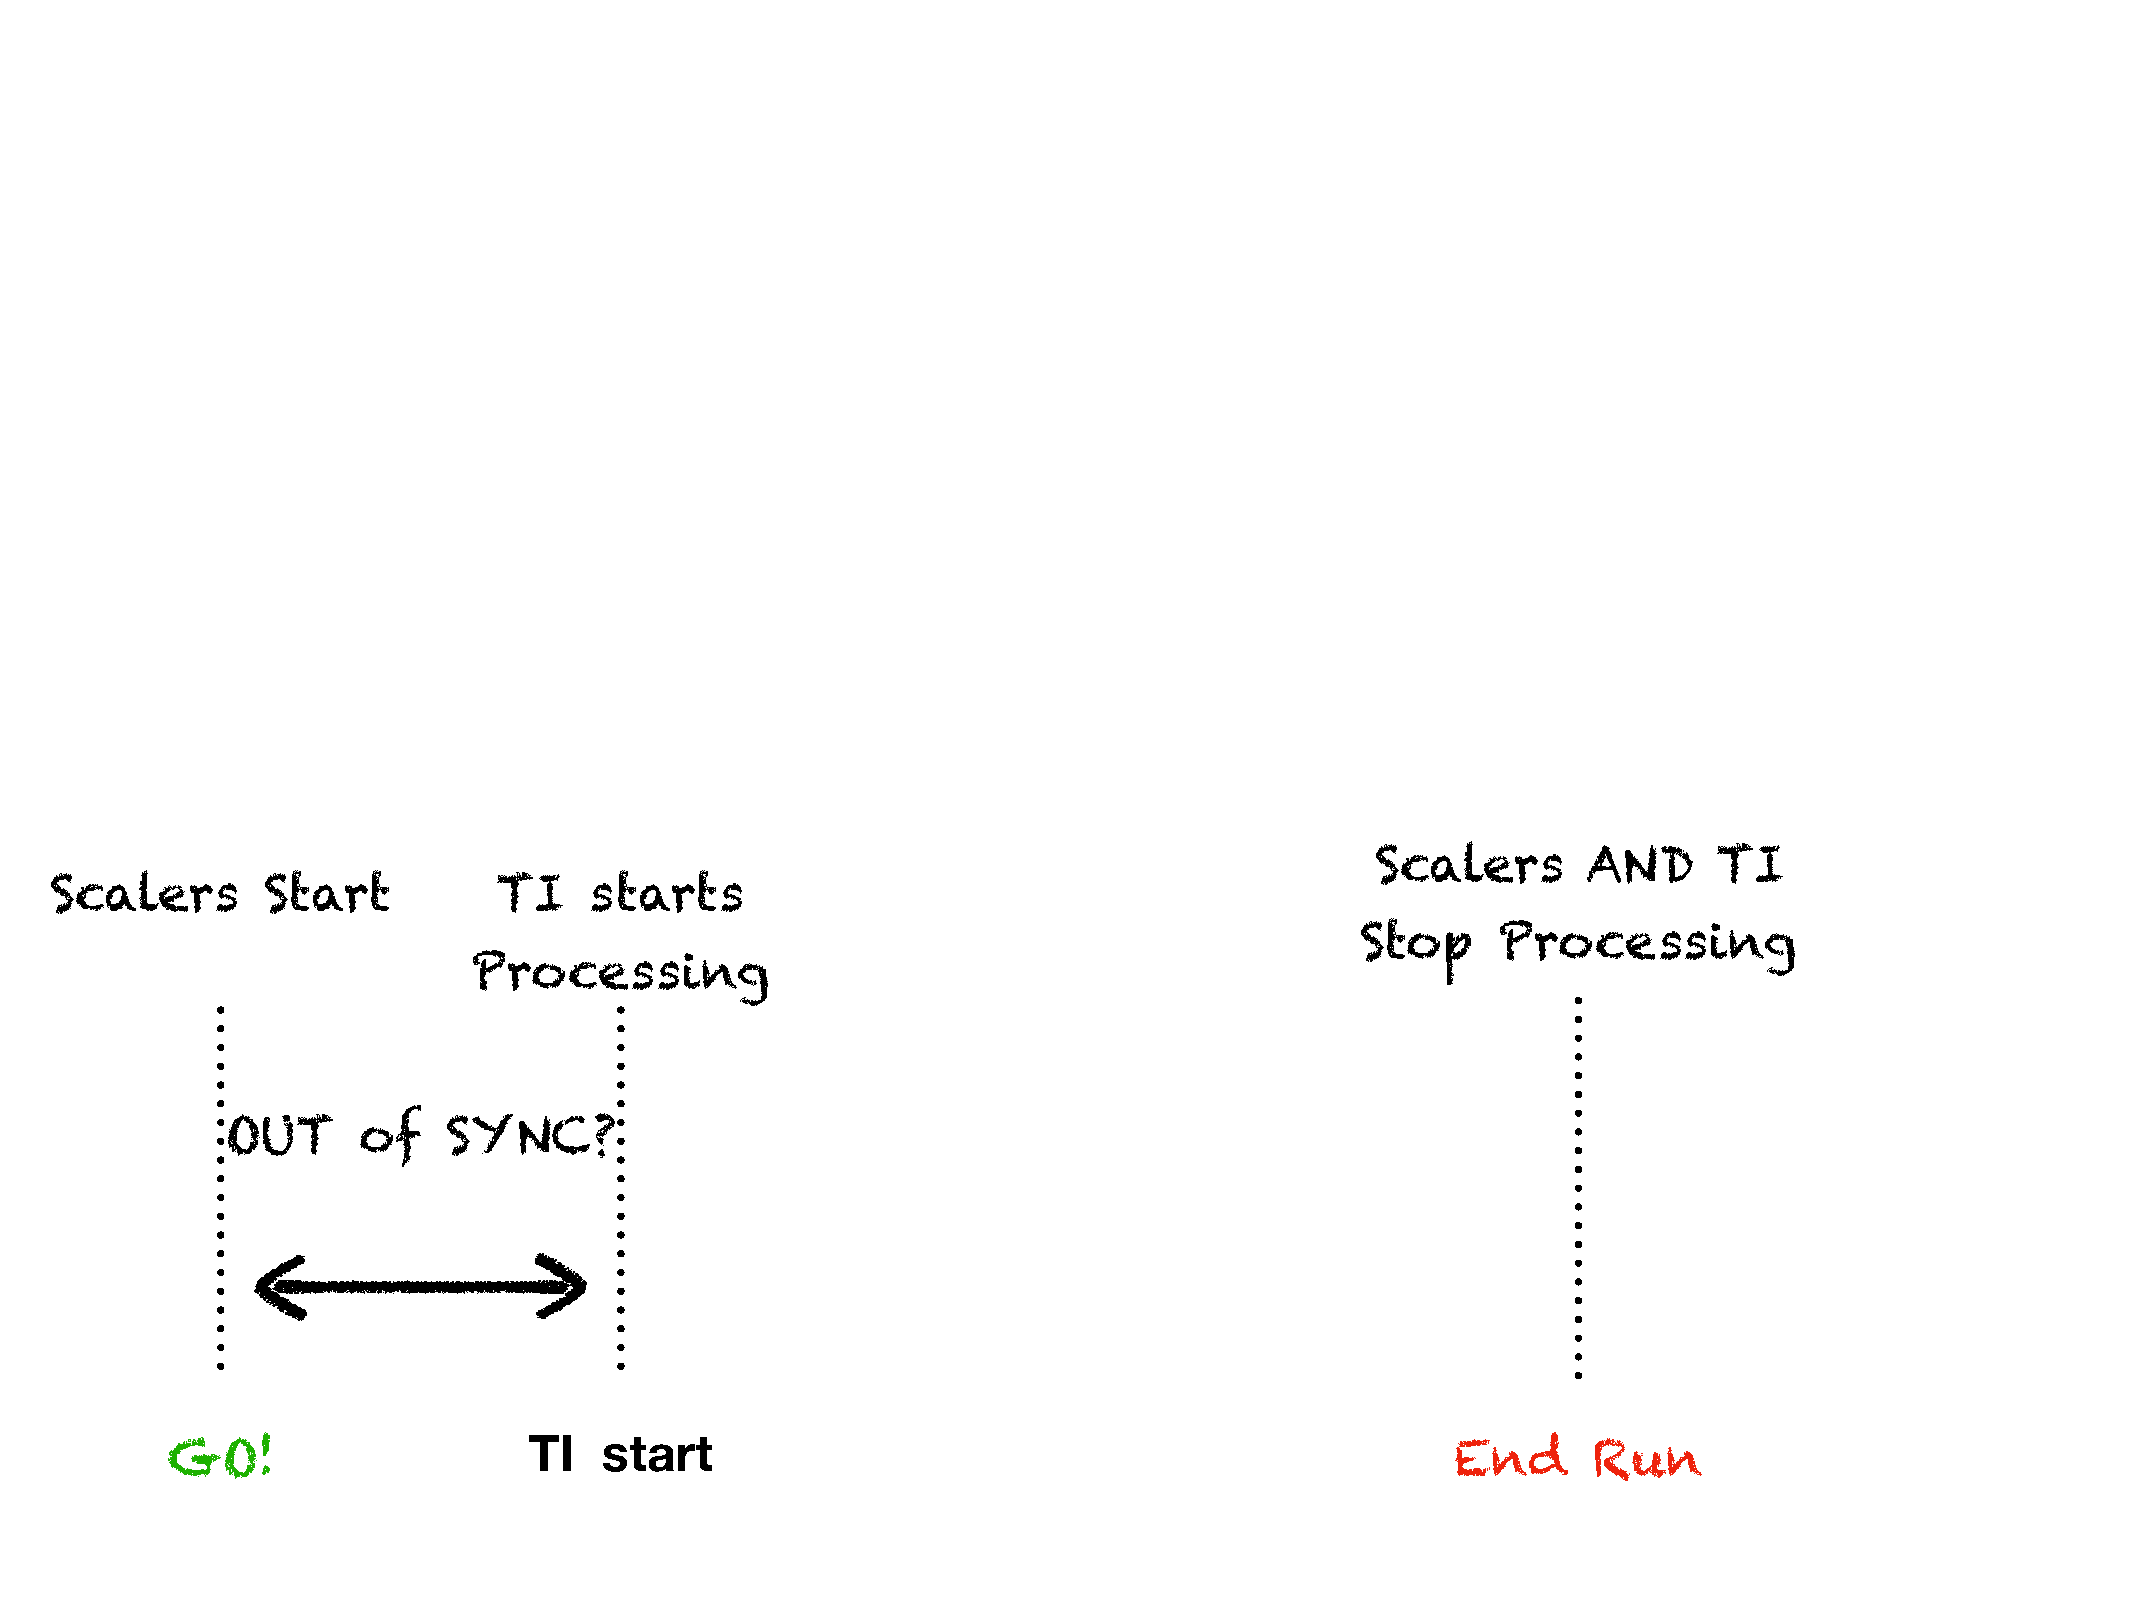
\includegraphics[width=3.4in, height=1.5in]{edtm/TI_Scaler_SYNC.pdf}
  \caption{Diagram showing unsynchronized TI and scaler modules.}
  \label{fig:TI_sync}
\end{figure}\\
When a run is started, a signal is sent to the TI module to initiate data processing, but the TI must also communicate with the scalers so that both
modules start counting simultaneously (in SYNC). The problem was that the TI and Scalers were not synchronized, so when a run was started, the scalers
would start counting events before the TI which caused a discrepancy in the live time calculations when a pulse generator was used. A second problem
was that the TI module internal scalers kept counting triggers after the END of run, which lead to an incorrect calculation of the computer live time
reported by the TI. \\
\indent These issues have been resolved, and the computer live time tests will continue on the near future to confirm that there are no other problems
with the live time calculations.
\section{D(e,e'p)n Experimental Run Plan}
\noindent My thesis subject, \textit{Deuteron Electro-Disintegration at Very High Missing Momenta} experiment is projected to run from February 26 to
March 3, 2018. The experiment consists of breaking the deuteron apart into a proton and neutron with an electron beam. The scattered electron and proton
will be detected by the SHMS and HMS, respectively, and the neutron will be reconstructed from mass-energy conservation laws. There will be a total of
five kinematics settings to be explored, two of which will be for spectrometer check and calibration purposes, and the other three settings will be the main
experimental settings that will explore the deuteron cross-section in unexplored regions of missing momentum with reduced final state interactions between
the proton and neutron. \\
\subsection{Spectrometer Settings: H(e,e'p) Scattering}
\noindent The first spectrometer setting will be to check that the spectrometers are pointing in the correct orientation in terms of angle and central
momentum. This is done via the elastic scattering of electrons off a 10 cm liquid Hydrogen target. In elastic scattering, e+p$\rightarrow$ e'+p, the
proton remains unchanged and re-scatters at a certain angle and momentum. By conservation laws, the final electron energy, $E'$, is determined to be
\begin{equation}\label{eq:h_elastic}
E'(\theta_{e}) = \frac{E_{e}}{1 + \frac{2E_{e}}{M_{p}}\sin^{2}\frac{\theta_{e}}{2}}
\end{equation}
where $E_{e}$ is the initial electron energy, $M_{p}$ is the proton mass and $\theta_{e}$ is the electron scattering angle. From Eq. \ref{eq:h_elastic},
once the electron angle, $\theta_{e}$ is determined, the electron scattering energy as well as the proton scattering angle and momentum, $\theta_{p}$ and $P_{p}$
are also fixed. The D(e,e'p)n kinematics at high missing momentum require the electron angle to be fixed at $\theta_{e}$= 12.189$^{o}$, as it is the most
sensitive kinematic variable to the cross sections we want to measure. This way, one does not run the risk of changing the SHMS spectrometer angle during the
experimental run. The kinematics are summarized in Table \ref{Table:h_elastic_kin}.
\begin{table}[ht]
\caption{Hydrogen Elastic Kinematics}
\centering
{\def\arraystretch{1.6}\tabcolsep=5pt
\begin{tabular}{c c c}
\hline\hline
\textbf{Spectrometer Settings} & \textbf{HMS} & \textbf{SHMS} \\ [0.5ex] % inserts table %heading
\hline
particles                  & protons & electrons \\
Central Angle (deg)        & 37.339 & 12.169  \\
Central Momentum (GeV/c)   & 2.938 & 8.700  \\ [1ex]
\hline
\end{tabular}
}
\label{Table:h_elastic_kin}
\end{table} \\
\subsection{Spectrometer Settings: D(e,e'p)n Kinematics}
The spectrometers will be set to measure D(e,e'p)n kinematics at low missing momentum setting first,
since there exist similar data from which we can compare results and apply any
corrections needed before exploring the high missing momentum region. Three high missing momentum values will then be explored,
each corresponding to a different HMS spectrometer setting. During the entire D(e,e'p)n runs, the SHMS spectrometer must stay at a
fixed angle and central momentumn. The SHMS settings for detecting electrons are:
\begin{table}[ht]
\caption{SHMS Central Kinematic Settings}
\centering
{\def\arraystretch{1.6}\tabcolsep=5pt
\begin{tabular}{c c}
\hline\hline
\textbf{Spectrometer Settings} & \textbf{SHMS} \\ [0.5ex] % inserts table %heading
\hline
particles detected                  & electrons \\
Central Angle (deg)        & 12.169  \\
Central Momentum (GeV/c)   & 8.700  \\ [1ex]
\hline
\end{tabular}
}
\label{Table:shms_d2_kin}
\end{table} \\
The HMS settings for detecting protons at low and high missing momentum of neutron are:
\begin{table}[ht]
\caption{HMS Central Kinematic Settings}
\centering
{\def\arraystretch{1.6}\tabcolsep=2pt
\begin{tabular}{c c c c c}
\hline\hline
\textbf{Spectrometer Settings} & \textbf{HMS} \\ [0.5ex] % inserts table %heading
\hline
particles  detected                &           &    protons &  \\
\hline
$P_{miss}$ (GeV/c)           & 0.08     &  0.500  & 0.650 & 0.800\\
$\theta_{HMS}$ (deg)       & 40.061   & 53.252    & 56.401 & 59.388  \\    
$P_{HMS}$ (GeV/c)            & 2.435    & 2.305    & 2.220 & 2.120  \\
\hline
\end{tabular}
}
\label{Table:hms_d2_kin}
\end{table} \\
\subsection{Reaction Kinematics}
\indent The true electron reaction kinematics differ from the spectrometer settings described in Tables
\ref{Table:h_elastic_kin} and \ref{Table:shms_d2_kin}. The kinematics for the scattered electron are
\begin{table}[ht]
\caption{Electron Kinematic Settings}
\centering
{\def\arraystretch{1.6}\tabcolsep=5pt
\begin{tabular}{c c c}
\hline\hline
& \textbf{H(e,e'p)} & \textbf{D(e,e'p)n} \\ [0.5ex] % inserts table %heading
\hline
$\theta_{e}$ (deg)    & 12.169 & 12.169 \\           
$P^{'}_{e}$  (GeV/c)   & 8.454 & 8.922 \\
\hline
\end{tabular}
}
\label{Table:elec_kin}
\end{table} \\
In going from Hydrogen to Deuteron kinematics in the experimental run plan, the electron
momentum actually increases as shown in table \ref{Table:elec_kin}. We could have chosen the
SHMS central momentum settings to match the reaction kinematics, however, changing the central
momentum settings from low to high momentum in the quadrupole magnets leads to a phenomenon
known as \textit{magnetic hysteresis}, which refers to the irreversibility of the magnetization process while ramping upthe current in the magnets. Due to this phenomenon, the central momentum
settings will have to be increased to above the established value due to a lagging of the
magnetization of a ferromagnetic material, such as iron in the quadrupoles \cite{hysteresis}. 
\subsection{ Monte Carlo Simulations on the Momentum Acceptance }
\noindent Since the central settings of the SHMS differ from the reaction kinematics, the detected particles are
offset from the center of the spectrometer momentum acceptance. A Monte Carlo simulation had to be done to verify
that the particles detected are within the spectrometer acceptance. For this purpose, events were randomly \textit{generated} over some large volume in which the spectrometer boundaries are defined. The \text{accepted} events landed within the
spectrometer boundaries (or phase space), each event with an equal probability or weight. The results are shown in Figure \ref{fig:h_elastics}. 
\begin{figure}[h!]
  \centering
  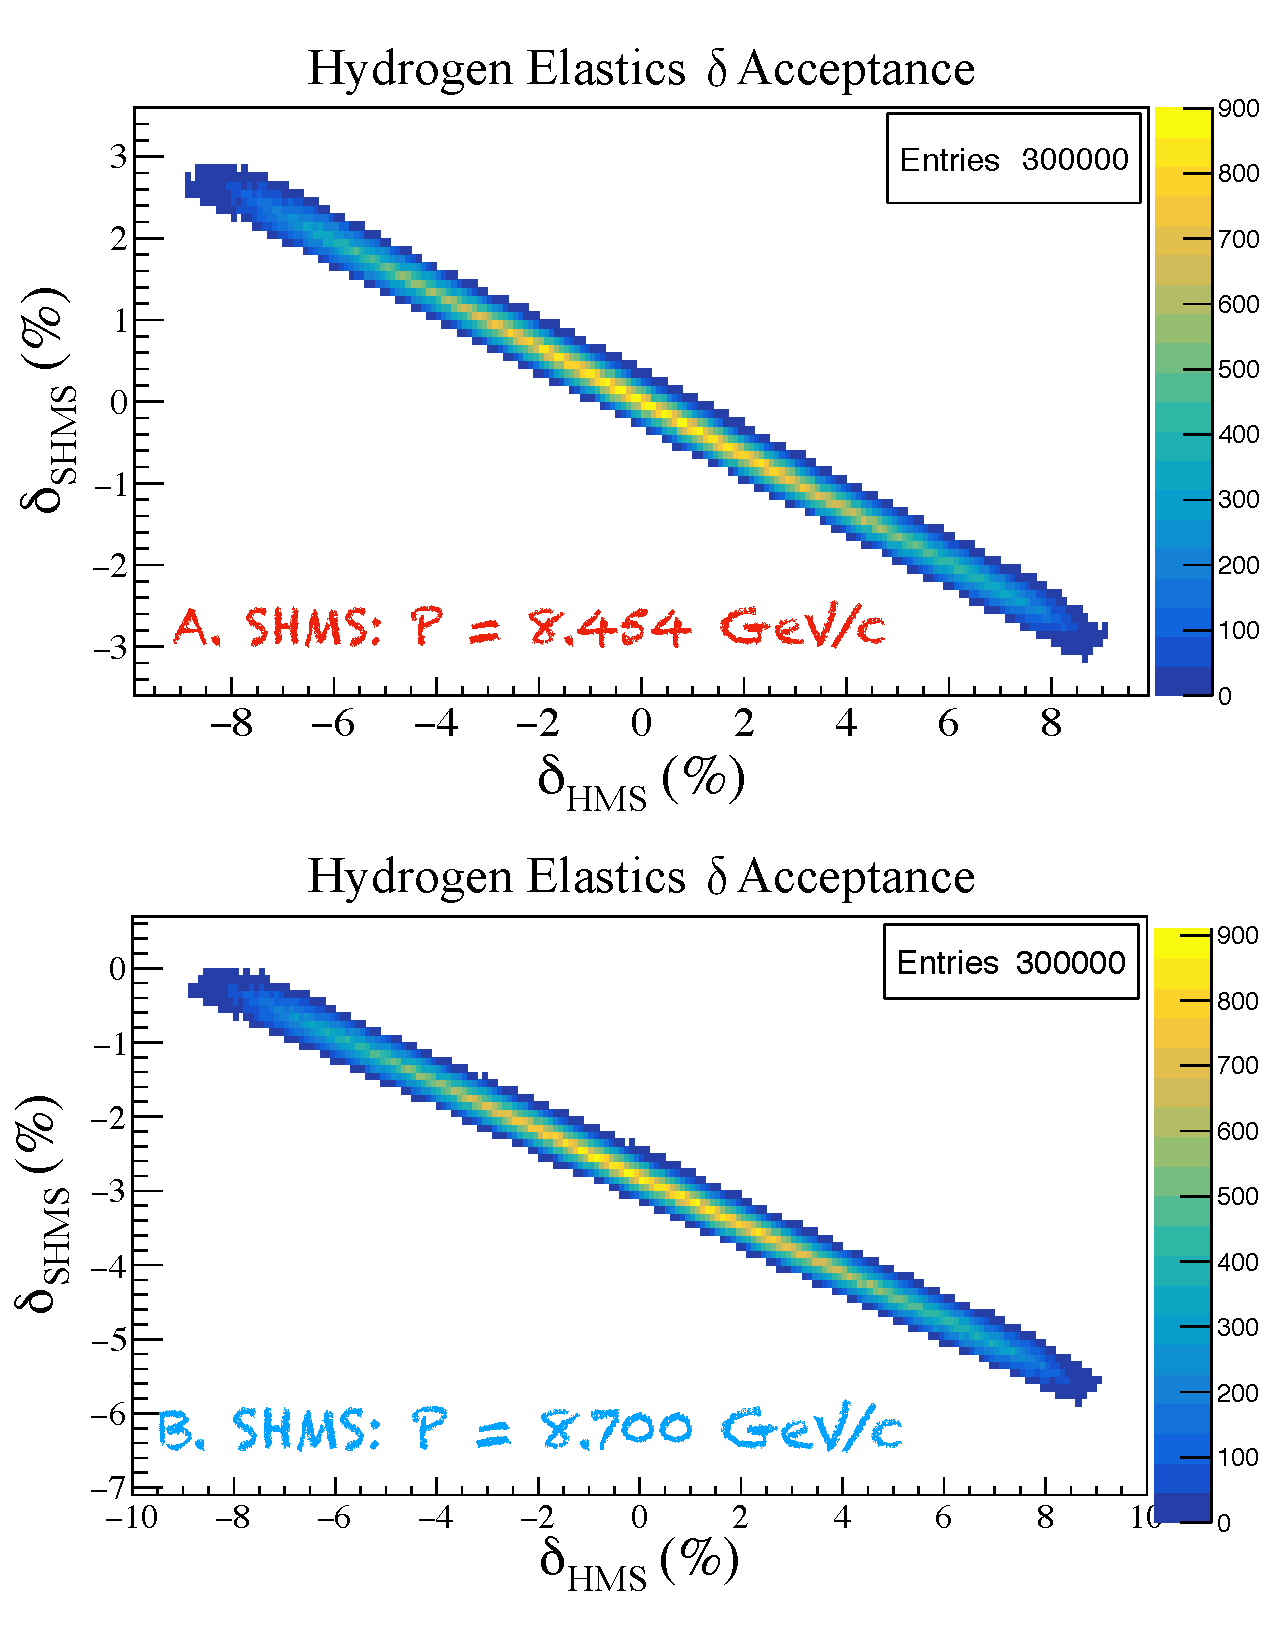
\includegraphics[width=3.3in, height=4.1in]{deut_kin/h_elast.pdf}
  \caption{Hydrogen Elastics simulation at difference central momenta.}
  \label{fig:h_elastics}
\end{figure} \\
The momentum acceptance is defined as
\begin{equation}
\delta = \frac{P - P_{0}}{P_{0}}
\end{equation}
where $P_{0}$ is the central momentum and $P$ is an arbitrary momentum within the acceptance. \\
\indent The Hydrogen elastics simulation results show that there is $\sim$3$\%$ shift in the SHMS momentum acceptance
if the central momentum were to be increased to 8.7 GeV/c. This means that the scattered electrons will now
be detected $3\%$ away from the center of the acceptance, which is not a significant offset given that the
full SHMS acceptance ranges from -10$\%$ to 25$\%$.
\indent A simulation was also done for the D(e,e'p)n reaction, where the central momentum of the SHMS was
also varied. The results are shown only for missing momentum $P_{miss}$ = 800 MeV/c.
\begin{figure}[h!]
  \centering
  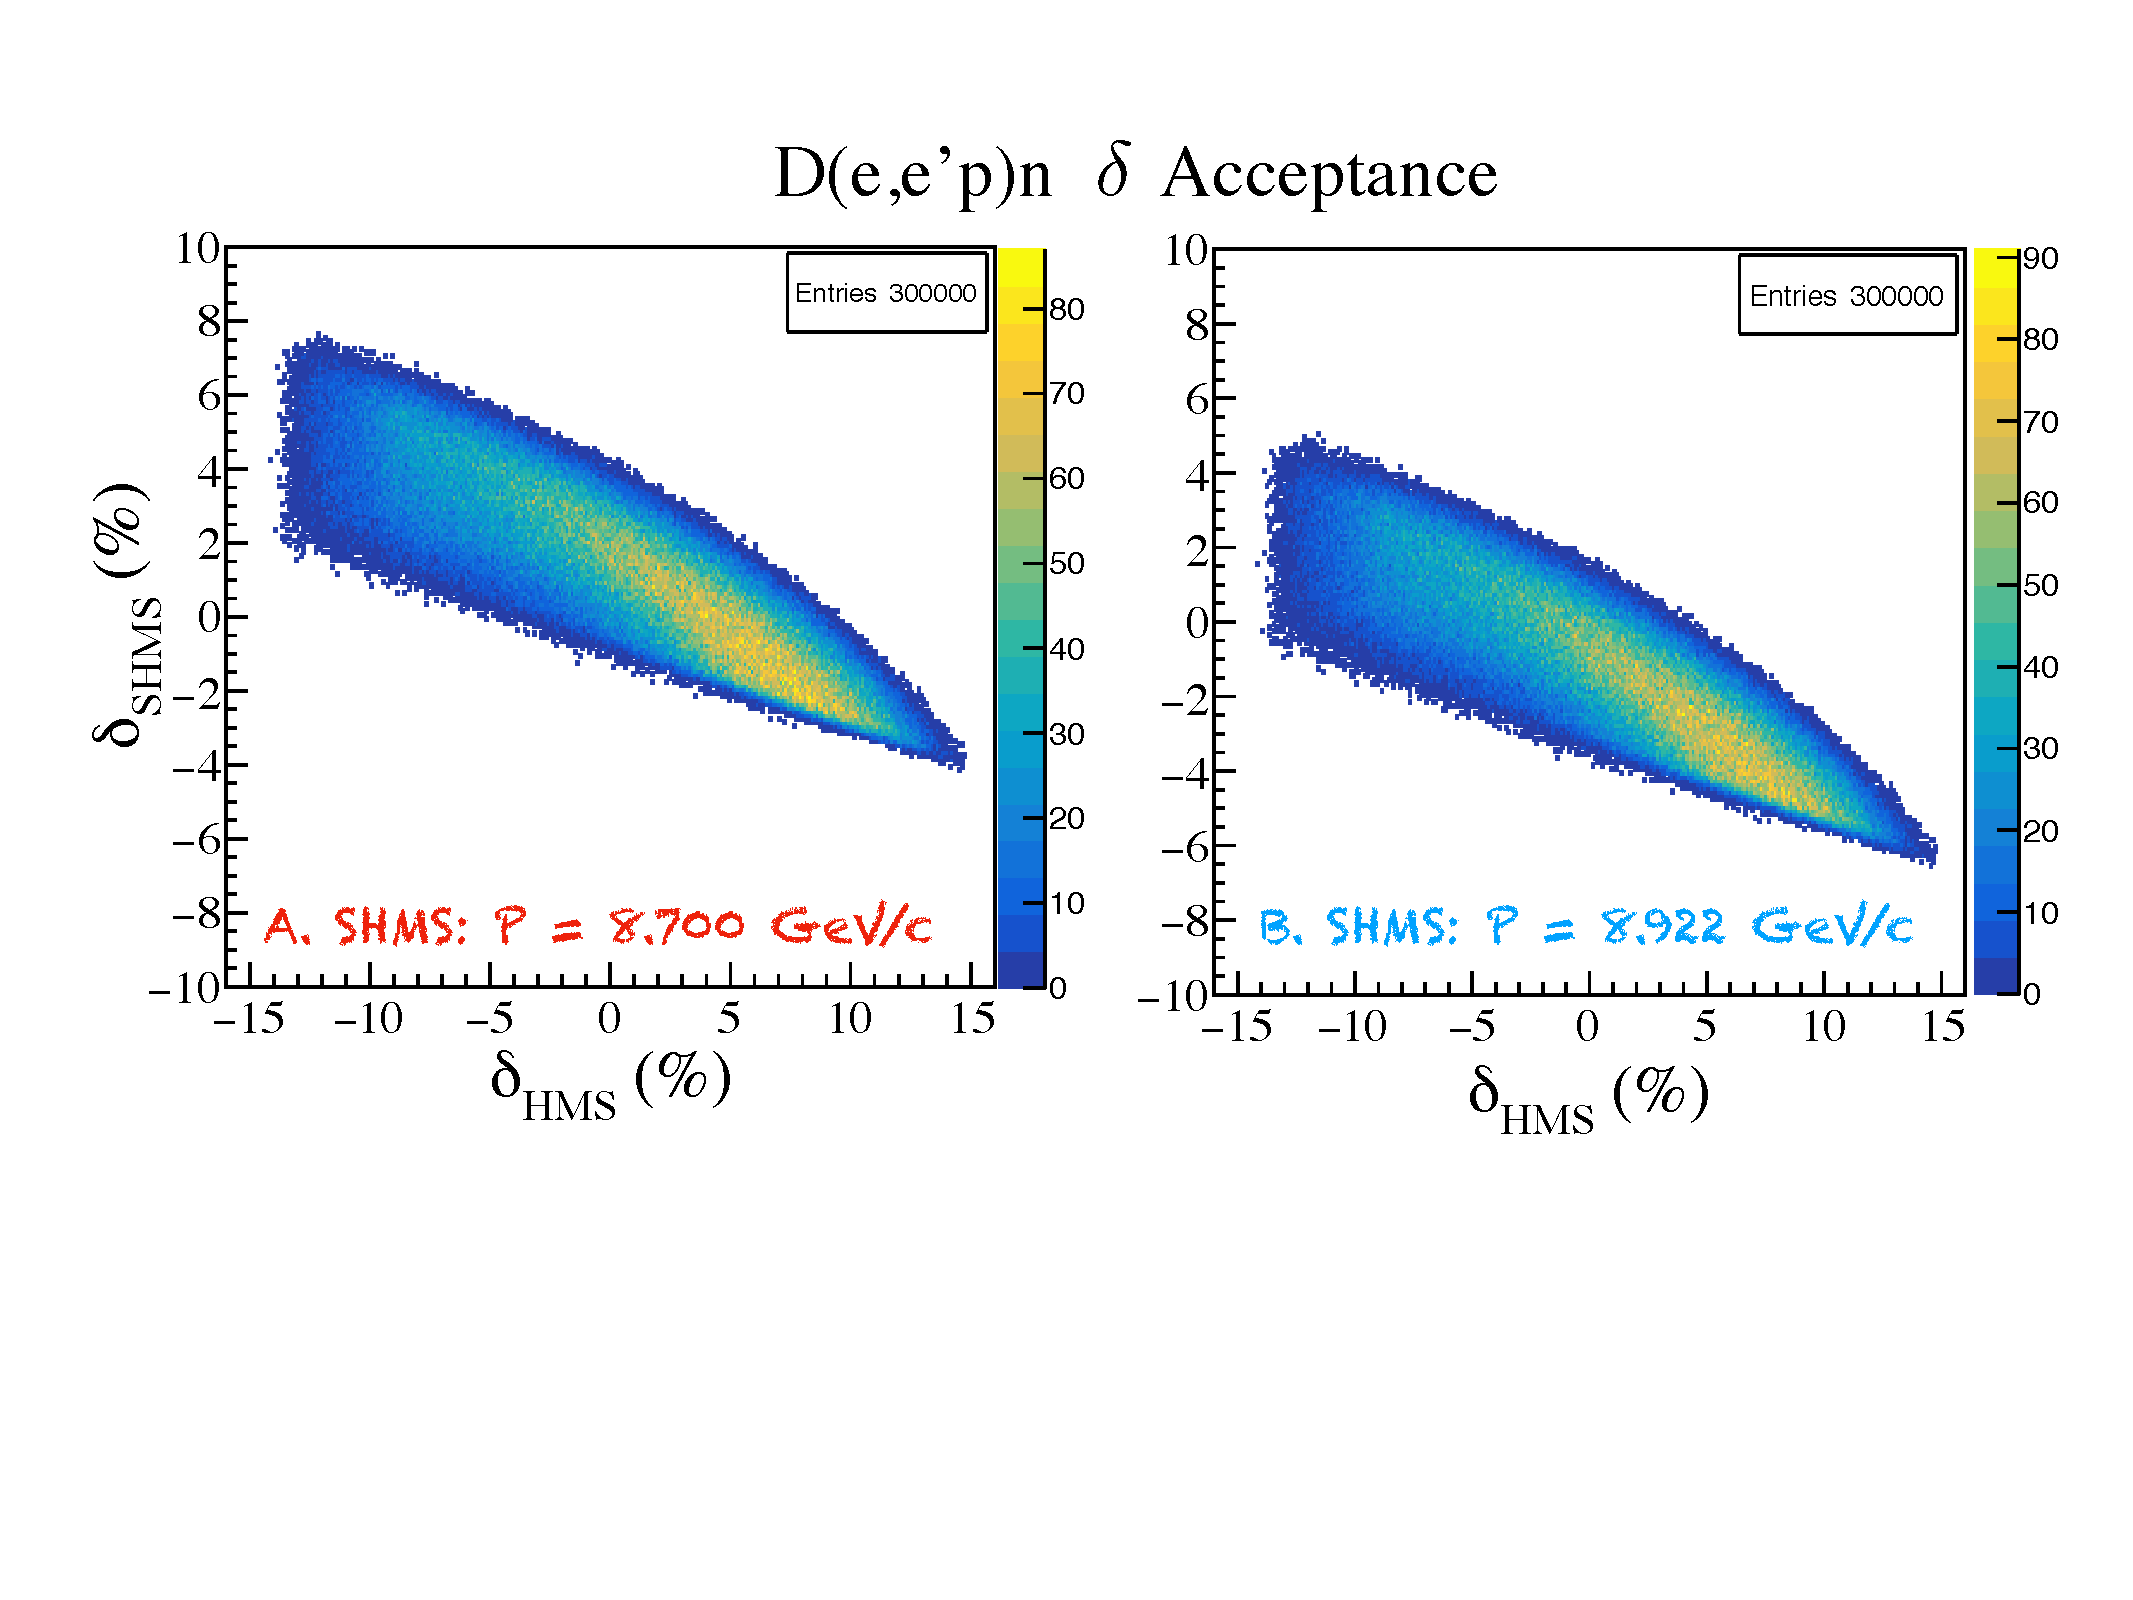
\includegraphics[width=3.5in, height=1.9in]{deut_kin/d2_acceptance.pdf}
  \caption{D(e,e'p)n simulation at missing momentum of 800 MeV/c, for two different SHMS central momentum settings.}
  \label{fig:deut_pmiss800}
\end{figure}
\indent From Figure \ref{fig:deut_pmiss800}, the majority of the electron-proton coincidence events represented by the yellow band
shifted by $\sim$ 2$\%$ towards the center of the SHMS acceptance when the central momentum was decreased to 8.7 GeV/c. Similar shifts
also occurred for the other momentum settings. \\
\indent The results from the simulations done on H(e,e'p) and D(e,e'p)n reactions demonstrate that by setting a common central momentum setting
of 8.7 GeV/c for the SHMS, the coincidence events are shifted by only $\sim$2$\%$ in the SHMS momentum acceptance.
\indent From the simulation results it has been determined that the SHMS should be set to a common central angle and momentum settings during the
entire experimental run, as the SHMS angle is the most sensitive to the D(e,e'p)n cross-section, changes in the central momentum setting would
lead to hysteresis in the magnets\cite{priv_comm}. 


\addtolength{\textheight}{-12cm}   % This command serves to balance the column lengths
                                  % on the last page of the document manually. It shortens
                                  % the textheight of the last page by a suitable amount.
                                  % This command does not take effect until the next page
                                  % so it should come on the page before the last. Make
                                  % sure that you do not shorten the textheight too much.

%%%%%%%%%%%%%%%%%%%%%%%%%%%%%%%%%%%%%%%%%%%%%%%%%%%%%%%%%%%%%%%%%%%%%%%%%%%%%%%%



%%%%%%%%%%%%%%%%%%%%%%%%%%%%%%%%%%%%%%%%%%%%%%%%%%%%%%%%%%%%%%%%%%%%%%%%%%%%%%%%



%%%%%%%%%%%%%%%%%%%%%%%%%%%%%%%%%%%%%%%%%%%%%%%%%%%%%%%%%%%%%%%%%%%%%%%%%%%%%%%%
\section*{ACKNOWLEDGMENT}
I would like to thank Drs. Werner Boeglin and Mark Jones for their constant support and guidance in writing this
paper. I would also like to give many thanks to Dr. Kavallieratos and the Nuclear Regulatory Commission Fellowship for supporting me throughout the Spring, Summer and Fall Terms of 2017.   

%\section*{APPENDIX}

%Appendixes should appear before the acknowledgment.


%%%%%%%%%%%%%%%%%%%%%%%%%%%%%%%%%%%%%%%%%%%%%%%%%%%%%%%%%%%%%%%%%%%%%%%%%%%%%%%%

%References are important to the reader; therefore, each citation must be complete and correct. If at all possible, references should be commonly available publications.


\newpage
\onecolumn
\bibliography{report.bib}
\bibliographystyle{ieeetr}






\end{document}
